\newcommand{\drpx}[1]{P_{#1}}
\newcommand{\comdrpx}[1]{P_{#1}^{com}}
\newcommand{\candrpx}[1]{P_{#1}^{can}}
\newcommand{\seqdrpx}[1]{P_{#1}^{seq}}

% \newcommand{\componentsx}[1]{CMPNTS(#1)}
% \newcommand{\componentsx}[1]{COMPONENTS(#1)}
% \newcommand{\componentsx}[1]{\text{\emph{COMPONENTS}}(#1)}
\newcommand{\componentsx}[1]{\textsc{Components}(#1)}

\newcommand{\Branch}{Branch}
\newcommand{\branch}{branch}
\newcommand{\branches}{branches}

% \newcommand{\branchx}[1]{\text{\emph{branch}}(#1)}
\newcommand{\branchx}[1]{\textsc{Branch}(#1)}
\newcommand{\branchGePG}{$\branchx{G,e,P_G}$}
\newcommand{\branchLfPL}{$\branchx{L,f,P_L}$}



\section{Main Result: Canonical DR-Plan, Optimality, and Algorithm}
\label{sec:DRP}
% In the problem of the optimal DR-Plan there is generally not a unique plan.
% % Indeed, we will prove a union of $N$ isostatic subgraphs will result in $N$ unique plans, but that at the $N^{\text{th}}$ level of the tree it will always be the same. Therefore, all choices of decomposition are in some sense equivalent. The theorem we seek to prove is thus:
% However, we will show that regardless of which children are chosen for the plan, so long as they satisfy the definition of an optimal DR-plan, the recombination will require solving of the same systems. Being the smallest such structure that offers this, the definition of an optimal DR-plan could be considered the canonical DR-plan.
% % To assist in showing this, we prove this core theorem throughout this section:

% In this section, we discuss 2D bar-joint graphs. All vertex weights are $2$, all edge weights are $1$, and constant $k= -{{3}\choose{2}}=-3$. Trivial graphs are a single vertex and empty set. Furthermore, 2D isostatic graphs must be connected.
% % The greatest density of a 2D isostatic graph is $-2$ (the vertex). The other disconnected part of the graph would need to have a density of $-1$, which is overconstrained and not possible in a isostatic graph (because there is no trivial graph with that density).


\subsection{Canonical DR-Plan}
In this section, we define a \dfn{canonical} plan to capture those aspects of an optimal DR-plan that mimic the  uniqueness of a complete DR-plan, and we show that the nonunique aspects do not affect optimality for independent (underconstrained or isostatic) graphs. Furthermore, we give an efficient \ComplexityCanDRP\ algorithm to find an optimal DR-plan of any independent graph.
% The definition is as follows:

In this section and in section~\ref{sec:recomb}, any reference to a graph $G$ without further specification is assumed to be isostatic (i.e.\ well-constrained or $(k,l)$-tight). Furthermore, we only consider unions and intersections of graphs that are induced subgraphs of a single parent graph $G$. In this case unions and intersections are well defined. For example, the union (resp.\ intersection) of $F_1 = (V_1, E_1)$ and $F_2 = (V_2, E_2)$ is the subgraph of $G$ induced by $V_1\cup V_2$ (resp.\ $V_1\cap V_2$).

% When using intersections and unions of graphs, we are always considering subgraphs of a single parent graph. In this case unions and intersections are well defined. For example, the union of $G_1=(V_1, E_1)$ and $G_2=(V_2, E_2)$ is the subgraph $(V_1\cup V_2, E_1\cup E_2)$; similarly, $G_1\cap G_2$ is the subgraph $(V_1\cap V_2, E_1\cap E_2)$.


% \begin{definition}\label{def:canonical_drplan}
%     The \dfn{canonical DR-plan} of a graph $G$ satisfies the following three properties:
%     (1) it is a DR-plan of $G$;
%     (2) children are rigid vertex-maximal proper subgraphs of the parent; and
%     (3) if all pairs of rigid vertex-maximal proper subgraphs intersect trivially then all of them are children, otherwise exactly two that intersect non-trivially are children.
% \end{definition}

\begin{definition}
[Canonical DR-plan]
\label{def:canonical_drplan}
    A \dfn{canonical DR-plan} is a DR-plan that satisfies the additional two properties:
    \begin{enumerate}
        \item \label{def:canonical_drplan:prop1} Children are rigid vertex-maximal proper subgraphs of the parent.
        \item \label{def:canonical_drplan:prop2} If all pairs of rigid vertex-maximal proper subgraphs intersect trivially then all of them are children, otherwise exactly two that intersect non-trivially are children.
    \end{enumerate}
\end{definition}

Definition~\ref{def:canonical_drplan} gives the canonical DR-plan a surprisingly strong Church-Rosser property, which is made explicit in Theorem~\ref{theorem:main}, the main result of this section.

\begin{theorem}
[Canonical is optimal]
\label{theorem:canonical_exists_and_is_optimal}
\label{theorem:canonical_is_optimal}
\label{theorem:main}
    A canonical DR-plan exists for a graph $G$ and any canonical DR-plan is optimal if $G$ is independent.
\end{theorem}


% \begin{theorem} \label{theorem:canonical_is_optimal}
%     \label{theorem:main}
%     Any canonical DR-plan is an optimal DR-plan.
% \end{theorem}

%The proof of this theorem is a direct consequence of the following  more general theorem.

%\begin{theorem}\label{theorem:main}
%Given an isostatic 2D bar-joint graph $G$ and ComDRP$(G)$, for all nodes $C$
%with children $C_1,\ldots,C_N$ preserve children according to the following rules.
%\begin{enumerate}
%    \item If $C_i \cap C_j$ is trivial then keep all $C_1,\ldots,C_N$ as children.
%    \item If $C_i \cap C_j$ is isostatic then select any two out of $C_1,\ldots,C_N$ as children.
%\end{enumerate}
%This is a canonical DR-plan.
%\end{theorem}


\begin{proof}
    We show the existence of a canonical DR-plan by constructing it as follows:

    Let $\comdrpx{G}$ be the complete DR-plan of the rigid 2D bar-joint graph $G$.
    % Begin with $\comdrp{G}$ of a rigid 2D bar-joint graph $G$.
    For all nodes $C$ with children $C_1,\ldots,C_N$ retain children nodes according to the following rules:
    \begin{enumerate}[(a)]
       \item \label{thm:main:proof:rule1} If $C_i \cap C_j$ is trivial then retain all $C_1,\ldots,C_N$ as children.
       \item \label{thm:main:proof:rule2} If $C_i \cap C_j$ is rigid then select any two out of $C_1,\ldots,C_N$ as children.
    \end{enumerate}

    This directly satisfies Properties (\ref{def:canonical_drplan:prop1}) and (\ref{def:canonical_drplan:prop2}) of a canonical DR-plan (see Definition~\ref{def:canonical_drplan}), because all the nodes in $\comdrpx{G}$ are rigid vertex-maximal proper subgraphs, which we shorten to \dfn{clusters}. To show that a canonical DR-plan is, in fact, a DR-plan:
    for Rule (\ref{thm:main:proof:rule1}) above, since we start with a complete DR-plan, if we preserve all the children it is still a DR-plan; for Rule (\ref{thm:main:proof:rule2}) above, we know that the union must be rigid as well and it cannot be anything other than $C$, otherwise we would have found a larger rigid proper subgraph of $C$, contradicting vertex-maximality.

    Note that if we begin with an isostatic graph, ``rigid'' can be replaced with ``isostatic'' throughout the construction and preserve the above properties. The rigid proper subgraphs of an isostatic graph must be isostatic themselves.

    Next we show that a canonical DR-plan is optimal.

    % First, note that any DR-plan $R$ without the Property (\ref{def:canonical_drplan:prop1}) of a canonical DR-plan can always be modified (by introducing intermediate nodes) to satisfy Property (\ref{def:canonical_drplan:prop1}) without increasing the max fan-in, since any rigid proper subgraph of a graph $C$ (a child of node $C$ of the DR-plan $R$) is the subgraph of some cluster of $C$.
    First, note that any DR-plan of $G$, $\drpx{G}$, without the Property (\ref{def:canonical_drplan:prop1}) of a canonical DR-plan can always be modified (by introducing intermediate nodes) to satisfy Property (\ref{def:canonical_drplan:prop1}) without increasing the max fan-in, since any child (a rigid proper subgraph) of node $C$ in $\drpx{G}$  is the subgraph of some cluster of $C$.
    Thus, without loss of generality, we can assume that an optimal DR-plan satisfies Property (\ref{def:canonical_drplan:prop1}) of a canonical DR-plan.

    The proof of optimality of a canonical DR-plan is by induction on its height. The base case trivially holds for canonical DR-plans of height 0, i.e.\ for single edges. The induction hypothesis is that canonical DR-plans of height $t$ are optimal for the root node.
    For the induction step consider a canonical DR-plan $\candrpx{C}$ rooted at node $C$ with height $t+1$.
    Notice that $\candrpx{C}$ contains a canonical DR-plan $\candrpx{C_i}$ for the graphs $C_i$ corresponding to each of $C$'s descendent nodes.
    Thus, from the induction hypothesis, we know that the $\candrpx{C_i}$ is optimal for $C_i$.

    To carry out the induction step, it is sufficient to demonstrate a set of nodes $S$ (of height at most $t$) that must be present in any DR-plan $\drpx{C}$ of graph $C$ that satisfies Property (\ref{def:canonical_drplan:prop1}), including a known optimal one; and furthermore, for any such DR-plan $\drpx{C}$, either (Claim 1) $S$ must be the set of children of $C$; or (Claim 2) for all the ancestors $A$ of $S$, $\drpx{A}$ has the minimum possible fan-in of 2 \todo{Shouldn't it be `node $A$ in $\drpx{C}$ has the minimum...'}.

    We show the two claims below.
    The first claim is that for a node $C$ whose clusters have trivial pairwise intersections, any DR-plan of $C$ that satisfies Property (\ref{def:canonical_drplan:prop1}) must also satisfy Property (\ref{def:canonical_drplan:prop2}) at $C$, i.e.\ the set of children $S$ of $C$ consists of all clusters of $C$.
    Because this is the only choice, it is the minimum fan-in at $C$ for any DR-plan for $C$ with Property (\ref{def:canonical_drplan:prop1}), including a known optimal one.
    The second claim shows that in the case of nodes $C$ whose rigid, vertex-maximal proper subgraphs have  non-trivial pairwise intersections, every canonical DR-plan of $C$ that uses any possible choice of two such subgraphs of $C$ as children results in a minimum possible fan-in of 2 in the ancestor nodes $A$ leading to the \emph{same maximal antichain $S$ of descendants $D$ of $C$}. The antichain is maximal in the partial order of rigid subgraphs of $C$ under containment. I.e.\ $S$ satisfies the property that every proper vertex-maximal rigid subgraph of $C$ is a superset of some $D$ in $S$; this follows from properties of maximal antichains that no element of $S$ is contained in the union of other elements of $S$; and the union of elements of $S$ is $C$. Thus any DR-plan that satisfies Property (\ref{def:canonical_drplan:prop1}) and hence contains two or more of the rigid vertex-maximal proper subgraphs of $C$ as children must also contain every element of $S$. The two claims complete the proof of the induction step and thus the proof that every canonical DR-plan is optimal.



     % We do this inductively on the l, beginning with the root node, showing that the rules are always the optimal choice.
    % by discussing each rule and proving inductively that this is the optimal choice at each level of the DR-plan tree, starting with the root node.


    % Now we show that this plan is optimal by considering the two cases. Observation \ref{lemma:union_intersection} shows that we do not have to consider anything other than the two cases stated in the construction.
     % the intersection of any two isostatic subgraphs can only result in trivial or isostatic subgraphs. Therefore, given $C$ and its isostatic vertex-maximal subgraphs $C_1,\ldots,C_N$, the are only two possibilities to considerthat a canonical DR-plan subgraphs $C_i$ and $C_j$ have a trivial intersection, or (2) they have an isostatic intersection.





    \medskip\noindent
    \vemph{Claim 1:}
    Let the set of clusters of node $C$ be $C_1,\ldots,C_N$. If the pairwise intersection of clusters is trivial, all of the clusters must be children of $C$ in an optimal DR-plan
    % A set of clusters $C_1,\ldots,C_N$ whose pairwise intersection is trivial must all be children of $C$ in an optimal DR-plan.

    We prove this claim by showing that the union of no subset of the children can be $C$, thereby requiring all of them to be included as children.

    We prove by contradiction.
    % Assume to the contrary that the strict subset $S\subsetneq \{1,\ldots,N\}$ such that $U=\bigcup_{i\in S}{C_i}$ is isostatic. If $U\neq C$, then we found a larger proper subgraph contradicting vertex-maximality of the $C_i$. So, it must be that $U=C$.
    % \usestwod
    % However, since $C_i \cap C_j$ is trivial then for $k\notin S$ we know, by Lemma \ref{lemma:combined_lemma}, Item \ref{lemma:uc_intersection_makes_all_uc}, $U\cap C_k$ must be one or more trivial, i.e.\ disconnected vertices. By definition of a DR-plan, $C_k=C\cap C_k$ and we know that $U=C$ so $C_k=U\cap C_k$. Thus, $C_k$ is (i) a collection of disconnected vertices, and (ii) an isostatic subgraph of $C$, which is impossible. As $C$ is isostatic, this means the union of no proper subset of $C_1,\ldots,C_N$ is isostatic, nor is it equal to $C$, proving Claim 1.
    Assume to the contrary that there is a strict subset $S$ of the clusters such that $U$, the union of all elements in $S$, is isostatic. If $U\neq C$, then we found a larger proper subgraph contradicting vertex-maximality of the clusters in set $S$. So, it must be that $U=C$.
    \usestwod
    However, since $C_i \cap C_j$ is trivial then for $C_k\notin S$ we know, by Lemma \ref{lemma:combined_lemma}, Item \ref{lemma:uc_intersection_makes_all_uc}, $U\cap C_k$ must be one or more vertices, i.e.\ disconnected trivial subgraphs. By definition of a DR-plan, $C_k=C\cap C_k$ and we know that $U=C$ so $C_k=U\cap C_k$. Thus, $C_k$ is (i) a collection of disconnected vertices, and (ii) an isostatic subgraph of $C$, which is impossible. As $C$ is isostatic, this means the union of no proper subset of $C_1,\ldots,C_N$ is isostatic, nor is it equal to $C$, proving Claim 1.

    Furthermore, since a canonical DR-plan has nodes with proper rigid \vemph{vertex-maximal} subgraphs as children, if, as in this case, their pairwise intersection is trivial, it follows that any node has at most as many children as a DR-plan without this restriction, because the union of the children must contain all edges of the parent. Therefore, the canonical DR-plan is the optimal choice in this case of trivial intersections.

    \medskip\noindent
    \vemph{Claim 2:}
    Let the set of clusters of node $C$ be $C_1,\ldots,C_N$. If some pair of clusters
    % If some pair in the set of clusters $C_1,\ldots,C_N$ of $C$
    has an isostatic (non-trivial) intersection, then choosing any two as children (minimum possible fan-in) will result in the same maximal antichain of descendants of node $C$.

    To prove Claim 2, notice that if $C_i\cap C_j$ is isostatic, then, by Observation \ref{lemma:union_intersection}, $C_i\cup C_j$ is also isostatic. This means that, by Lemma \ref{lemma:combined_lemma}, Point \ref{lemma:wc_intersection_makes_all_wc}, the union of any two children of $C$ is $C$ itself. Thus, any two children can be chosen to make a canonical DR-plan and that is the minimum fan-in possible for a node of the DR-plan.

    \newcommand{\induceonc}[1]{Idc\left(C,#1\right)}
    \renewcommand{\induceonc}[1]{#1}
    \newcommand{\iunion}[1]{\induceonc{I\cup\bigcup_{k\in [N]\setminus\{#1\}}{R_k}}}

    However, to guarantee that any two are the \vemph{optimal} choice, it must ensure minimum fan-in over all descendants leading up to a common maximal antichain $S$ of subgraphs.

    % To prove this holds, take the set $[N]=\{1,\dots,N\}$, and denote $I=\bigcap_{k\in [N]}{C_k}$ and $R_k=C\setminus C_k$. Suppose  $C_i$ and $C_j$, where $i\neq j$,  are  the children. For convenience, we will assume all subgraphs are induced subgraphs of $C$. We know that $C=\induceonc{I\cup\bigcup_{k\in [N]}{R_k}}$ and $C_i=\iunion{i}$. The isostatic vertex-maximal subgraphs of $C_i$ are $(\iunion{i,1}),\ldots,(\iunion{i,i-1}),(\iunion{i,i+1}),\ldots,(\iunion{i,N})$ all of whose pairwise intersections are isostatic subgraphs. So any two of these are viable children for $C_i$.
    Let $I$ denote the intersection of all the clusters; we call this the \dfn{core}. Let $R_i$ be the graph induced by the edge set of $C$ minus the edge set of $C_i$; we call these the \dfn{appendages}.\footnote{\dfn{Core} and \dfn{appendage} are used in Section~\ref{sec:DRP:algo} and are more formally defined in Definition~\ref{def:seqdrp}.} Note that $C$ is the core plus all appendages, and cluster $C_i$ is the core plus all appendages except $R_i$.
    % To prove this holds,
    Suppose $C_i$ and $C_j$, where $i\neq j$, are taken to be the children of node $C$.
    % We know that $C=\induceonc{I\cup\bigcup_{k\in [N]}{R_k}}$ and $C_i=\iunion{i}$.
    The $N-1$ clusters of $C_i$ are the core plus all appendages except $R_i$ and $R_j$, for each $j\neq i$. The pairwise intersection of any of these clusters of $C_i$ will clearly be isostatic, so any two of them are viable children of node $C_i$.
     % $(\iunion{i,1}),\ldots,(\iunion{i,i-1}),(\iunion{i,i+1}),\ldots,(\iunion{i,N})$ all of whose pairwise intersections are isostatic subgraphs. So any two of these are viable children for $C_i$.
    % Since
    % \[C_i=Idc\left(C,I\cup\bigcup_{k\in S_N\setminus\{i\}}{R_k}\right)\]
    % the children of $C_i$ will be
    % \[Idc\left(C,I\cup\bigcup_{k\in S_N\setminus\{i,m\}}{R_k}\right)\]
    % and
    % \[Idc\left(C,I\cup\bigcup_{k\in S_N\setminus\{i,n\}}{R_k}\right)\]
    % % $C_i=Idc\left(C,I\cup\bigcup_{k\in S_N\setminus\{i\}}{R_k}\right)$
    % % the children of this node will be
    % % $Idc\left(C,I\cup\bigcup_{k\in S_N\setminus\{i,m\}}{R_k}\right)$
    % % and
    % % $Idc\left(C,I\cup\bigcup_{k\in S_N\setminus\{i,n\}}{R_k}\right)$
    % for arbitrary $m$ and $n$, where $i,j,m,n$ do not equal each other. \todo{Prove these are valid children? Or is this obvious?}
    Beginning with node $C$, this pattern repeats for $N-1$ levels. Every node in this subtree rooted at $C$ has a fan-in of two (the minimum possible) up through this level. At level $N-1$, we have a set of nodes where each node is the core plus some appendage (with every appendage appearing at least once).
    % This continues for $N-1$ levels, always with fan-in of two (the minimum possible), at which point every descendant of $C$ is some $\induceonc{I\cup R_k}$ for $k\in [N]$, with every $k$ appearing at least once.
    % At the last level, there are exactly two rigid proper vertex-maximal subgraphs, and hence a unique choice of pair of children.
    Thus, regardless of the sequence of choices of $C_i$ and $C_j$, and of their descendants at each level, the DR-plan has the optimal fan-in of two for every node for $N-1$ levels, and the collection of last level nodes contain the same maximal antichain of subgraphs (for all choices).
    %
    % \medskip\noindent
    % This proof then applies to itself recursively to show that the fan-in of the children will also be minimum.
    %
    % -- say this at top `proof is by induction on the level of the dr=plan'
\end{proof}

This proof of this theorem relies on the following crucial observation and lemma. These will be used again in the application sections (\ref{sec:bodypin} and \ref{sec:pinnedline}) of the paper, with modifications to work for other types of qusecs.

\begin{observation*}
\label{lemma:union_intersection}
    If $F_i$ and $F_j$ are isostatic subgraphs of an independent graph then the following hold:
    % \begin{enumerate}
    %     \item $F_i\cup F_j$ is not trivial.
    %     \item $F_i\cup F_j$ is underconstrained if and only if $F_i\cap F_j$ is trivial.
    %     \item $F_i\cup F_j$ is isostatic if and only if $F_i\cap F_j$ is isostatic.
    %     \item $F_i\cap F_j$ is not underconstrained.
    % \end{enumerate}
    (1) $F_i\cup F_j$ is not trivial;
    (2) $F_i\cup F_j$ is underconstrained if and only if $F_i\cap F_j$ is trivial;
    (3) $F_i\cup F_j$ is isostatic if and only if $F_i\cap F_j$ is isostatic; and
    (4) $F_i\cap F_j$ is not underconstrained.
\end{observation*}

The following key properties hold at the nodes of a canonical DR-plan.

\begin{lemma*}
\label{lemma:combined_lemma}
    Let $C$ be an isostatic node of a canonical DR-plan with distinct children $C_1,C_2,\ldots, C_N$. Assume $i\ne j$.
    Then
    \begin{enumerate}
        \item\label{lemma:wc_intersection_is_C}
        $C_i\cup C_j$ is isostatic if and only if $C_i\cup C_j = C$.

        \item\label{lemma:wc_intersection_makes_all_wc}
        If $C_i\cup C_j$ is isostatic, then $\forall k: C_i\cup C_k$ is isostatic. Alternatively, if $C_i\cup C_j=C$, then $\forall k: C_i\cup C_k=C$.

        \item\label{lemma:uc_intersection_makes_all_uc}
        If $C_i\cap C_j$ is trivial, then $\forall k: C_i\cap C_k$ is trivial.
    \end{enumerate}
\end{lemma*}

\begin{remark}
    The first item in the above lemma generalizes to the union of any number of children, $C_1,\ldots,C_k$, resulting in the desirable property of \dfn{cluster minimality} (defined in \cite{hoffman2001decompositionI} and in Section \ref{sec:prev}) holding for canonical-optimal DR-plans.
\end{remark}





% \begin{figure*}\centering
% \begin{subfigure}{.3\linewidth}\centering
%     % \newcommand{\tedge}[5]{\draw[#3] (#1)-- node[e, #5] (e#4) {#4} (#2)}

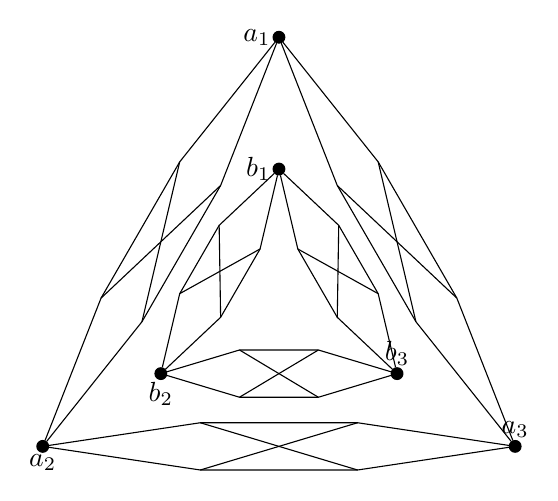
\begin{tikzpicture}[scale=3]
    \tikzstyle{v}=[draw, circle, minimum size=0.75cm]
    \tikzstyle{c}=[draw, circle, inner sep=1.5, fill=black]
    \tikzstyle{e}=[]

    \node[circle,fill=white,inner sep=7] (center) at (0,0-.125-.1) {};

    \node[c] (v1) at (0,0.866) [label={left,inner sep=.555}:$a_1$]{};
    \node[c] (v2) at (-1,-0.866) [label={below,inner sep=.555}:$a_2$]{};
    \node[c] (v3) at (1,-0.866) [label={above,inner sep=.555}:$a_3$]{};

    \node[c] (v4) at (0,0.433-.125) [label={left,inner sep=.555}:$b_1$]{};
    \node[c] (v5) at (-0.5,-0.433-.125) [label={below,inner sep=.555}:$b_2$]{};
    \node[c] (v6) at (0.5,-0.433-.125) [label={above,inner sep=.555}:$b_3$]{};

    \tedge{v1}{v2}{solid}{}{};
    \tedge{v1}{v3}{solid}{}{};
    \tedge{v2}{v3}{solid}{}{};

    \tedge{v4}{v5}{solid}{}{};
    \tedge{v4}{v6}{solid}{}{};
    \tedge{v5}{v6}{solid}{}{};


    \tedge{v1}{v4}{solid}{}{};
    \tedge{v2}{v5}{solid}{}{};
    \tedge{v3}{v6}{solid}{}{};


    \tedge{v4}{center}{dashed}{}{};
    \tedge{v5}{center}{dashed}{}{};
    \tedge{v6}{center}{dashed}{}{};


    % sin(30deg) = 0.5
    % cos(30deg) = 0.866

    % o/i -> outside/inside triangle
    % b/l/r -> bottom/left/right edge of triangle

    \coordinate (ob0) at (-0.333,-0.866-0.1);
    \coordinate (ob1) at (0.333,-0.866-0.1);
    \coordinate (ob2) at (-0.333,-0.866+0.1);
    \coordinate (ob3) at (0.333,-0.866+0.1);
    \draw (v2) -- (ob0) -- (ob1) -- (v3);
    \draw (v2) -- (ob2) -- (ob3) -- (v3);
    \draw (ob0) -- (ob3);
    \draw (ob2) -- (ob1);

    \draw[rotate around={60:(-1,-0.866)}] (v2) -- (-0.333,-0.766) -- (0.333,-0.766) -- (v1);
    \draw[rotate around={60:(-1,-0.866)}]  (v2) -- (-0.333,-0.966) -- (0.333,-0.966) -- (v1);
    \draw[rotate around={60:(-1,-0.866)}]  (-0.333,-0.766) -- (0.333,-0.966);
    \draw[rotate around={60:(-1,-0.866)}]  (-0.333,-0.966) -- (0.333,-0.766);

    \draw[rotate around={-60:(1,-0.866)}] (v3) -- (0.333,-0.766) -- (-0.333,-0.766) -- (v1);
    \draw[rotate around={-60:(1,-0.866)}]  (v3) -- (0.333,-0.966) -- (-0.333,-0.966) -- (v1);
    \draw[rotate around={-60:(1,-0.866)}]  (-0.333,-0.766) -- (0.333,-0.966);
    \draw[rotate around={-60:(1,-0.866)}]  (-0.333,-0.966) -- (0.333,-0.766);




    \coordinate (ib0) at (-0.167,-0.433-.125-0.1); %(-.167,-.658)
    \coordinate (ib1) at (0.167,-0.433-.125-0.1); %(.167,-.658)
    \coordinate (ib2) at (-0.167,-0.433-.125+0.1);%(-.167,-.458)
    \coordinate (ib3) at (0.167,-0.433-.125+0.1);%(.167,-.458)
    \draw (v5) -- (ib0) -- (ib1) -- (v6);
    \draw (v5) -- (ib2) -- (ib3) -- (v6);
    \draw (ib0) -- (ib3);
    \draw (ib2) -- (ib1);

    \draw[rotate around={60:(-0.5,-0.558)}] (v5) -- (-.167,-.658) -- (.167,-.658) -- (v4);
    \draw[rotate around={60:(-0.5,-0.558)}]  (v5) -- (-.167,-.458) -- (.167,-.458) -- (v4);
    \draw[rotate around={60:(-0.5,-0.558)}]  (-.167,-.658) -- (.167,-.458);
    \draw[rotate around={60:(-0.5,-0.558)}]  (-.167,-.458) -- (.167,-.658);

    \draw[rotate around={-60:(0.5,-0.558)}] (v6) -- (.167,-.658) -- (-.167,-.658) -- (v4);
    \draw[rotate around={-60:(0.5,-0.558)}]  (v6) -- (.167,-.458) -- (-.167,-.458) -- (v4);
    \draw[rotate around={-60:(0.5,-0.558)}]  (-.167,-.658) -- (.167,-.458);
    \draw[rotate around={-60:(0.5,-0.558)}]  (-.167,-.458) -- (.167,-.658);
% \newcommand{\tedge}[5]{\draw[#3] (#1)-- node[e, #5] (e#4) {#4} (#2)}

    % \draw (-1,-0.866) -- (-0.333,-0.966);

\end{tikzpicture}

%     \caption{}\label{fig:c2c3ofk33s:a}
% \end{subfigure}%
% \begin{subfigure}{.7\linewidth}\centering
%     % \newcommand{\tedge}[5]{\draw[#3] (#1)-- node[e, #5] (e#4) {#4} (#2)}

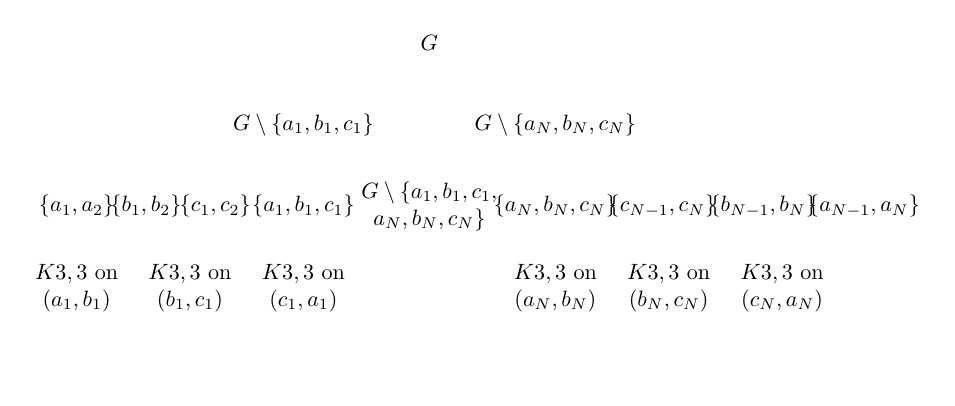
\begin{tikzpicture}[scale=.8, transform shape]
    \tikzstyle{v}=[draw, circle, minimum size=0.75cm, font=\footnotesize]
    % \tikzstyle{b}=[draw, font=\footnotesize]
    \tikzstyle{b}=[align=center]
    \tikzstyle{e}=[]

    \node[b] (c0) at (0,0*1.3) {$G$};
    \node[b] (c1a) at (-2,-1*1.3) {$G\setminus\{a_1,b_1,c_1\}$};
    \node[b] (c1b) at (2,-1*1.3) {$G\setminus\{a_N,b_N,c_N\}$};
    \node[b] (c2b) at (0,-2*1.3) {$G\setminus\{a_1,b_1,c_1,$ \\ $a_N,b_N,c_N\}$};
    \node[b] (c2a) at (-2,-2*1.3) {$\{a_1,b_1,c_1\}$};
    \node[b] (c2c) at (2,-2*1.3) {$\{a_N,b_N,c_N\}$};
    \node[b] (c2ab1) at (-5.6,-2*1.3) {$\{a_1,a_2\}$};
    \node[b] (c2ab2) at (-4.5,-2*1.3) {$\{b_1,b_2\}$};
    \node[b] (c2ab3) at (-3.4,-2*1.3) {$\{c_1,c_2\}$};
    \node[b] (c2bc1) at (6.9,-2*1.3) {$\{a_{N-1},a_N\}$};
    \node[b] (c2bc2) at (5.3,-2*1.3) {$\{b_{N-1},b_N\}$};
    \node[b] (c2bc3) at (3.7,-2*1.3) {$\{c_{N-1},c_N\}$};

    \node[b] (ab1k33) at (-5.6,-3*1.3) {$K3,3$ on \\ $(a_1,b_1)$};
    \node[b] (bc1k33) at (-7.6/2,-3*1.3) {$K3,3$ on \\ $(b_1,c_1)$};
    \node[b] (ca1k33) at (-2,-3*1.3) {$K3,3$ on \\ $(c_1,a_1)$};

    \node[b] (abNk33) at (2,-3*1.3) {$K3,3$ on \\ $(a_N,b_N)$};
    \node[b] (bcNk33) at (7.6/2,-3*1.3) {$K3,3$ on \\ $(b_N,c_N)$};
    \node[b] (caNk33) at (5.6,-3*1.3) {$K3,3$ on \\ $(c_N,a_N)$};


    \node[b] (c3a) at (-2,-4*1.3) {};
    \node[b] (c3b) at (2,-4*1.3) {};


    \tedge{c0}{c1a}{solid}{}{};
    \tedge{c0}{c1b}{solid}{}{};

    \tedge{c1a}{c2ab1}{solid}{}{};
    \tedge{c1a}{c2ab2}{solid}{}{};
    \tedge{c1a}{c2ab3}{solid}{}{};
    \tedge{c1a}{c2a}{solid}{}{};
    \tedge{c1a}{c2b}{solid}{}{};

    \tedge{c1b}{c2bc1}{solid}{}{};
    \tedge{c1b}{c2bc2}{solid}{}{};
    \tedge{c1b}{c2bc3}{solid}{}{};
    \tedge{c1b}{c2b}{solid}{}{};
    \tedge{c1b}{c2c}{solid}{}{};

    \tedge{c2a}{ab1k33}{solid}{}{};
    \tedge{c2a}{bc1k33}{solid}{}{};
    \tedge{c2a}{ca1k33}{solid}{}{};
    \tedge{c2c}{abNk33}{solid}{}{};
    \tedge{c2c}{bcNk33}{solid}{}{};
    \tedge{c2c}{caNk33}{solid}{}{};

    \tedge{c2b}{c3a}{dashed}{}{};
    \tedge{c2b}{c3b}{dashed}{}{};
\end{tikzpicture}

%     \caption{}\label{fig:c2c3ofk33s:b}
% \end{subfigure}

% \caption{(\ref{fig:c2c3ofk33s:a}) A doublet ($C_2 \times C_3$) with each edge of the triangles replaced by a $K_{3,3}$. This pattern continues inwards for a total of $N$ triangles, indicated by the dashed lines. (\ref{fig:c2c3ofk33s:b}) Most of the DR-plan of this graph, omitting further decomposition of $K_{3,3}$ subgraphs into the separate 9 edges and of edges into the component nodes. $G\setminus\{a_i,b_i,c_i\}$ is shorthand for $G$ difference those nodes and all of the nodes in the corresponding $K_{3,3}$ subgraphs. The dashed lines indicated that this exact structure is repeated.}
% \label{fig:c2c3ofk33s}
% \end{figure*}


% \FigInit
%     {(\ref{fig:c2c3ofk33s:a}) A doublet ($C_2 \times C_3$) with each edge of the triangles replaced by a $K_{3,3}$. This pattern continues inwards for a total of $N$ triangles, indicated by the dashed lines. (\ref{fig:c2c3ofk33s:b}) Most of the DR-plan of this graph, omitting further decomposition of $K_{3,3}$ subgraphs into the separate 9 edges and of edges into the component nodes. $G\setminus\{a_i,b_i,c_i\}$ is shorthand for $G$ difference those nodes and all of the nodes in the corresponding $K_{3,3}$ subgraphs. The dashed lines indicated that this exact structure is repeated.}
%     {fig:c2c3ofk33s}
% \FigTwoSubfigWithWidth
%     {.3}
%     {../../img/epsfromtikz/c2c3_of_k33s-0}
%     {}
%     {fig:c2c3ofk33s:a}
%     %
%     {.7}
%     {../../img/epsfromtikz/c2c3_of_k33s-1}
%     {}
%     {fig:c2c3ofk33s:b}


% \ClearMyMinHeight
% \SetMyMinHeight{.3}{../../img/epsfromtikz/c2c3_of_k33s-0}
% \SetMyMinHeight{.7}{../../img/epsfromtikz/c2c3_of_k33s-1}

% \begin{figure*}\centering%
%     %
%     \begin{subfigure}{0.3\linewidth}\centering
%         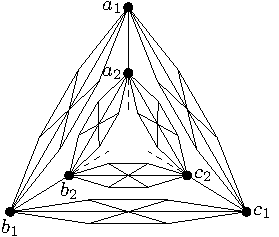
\includegraphics[height=\myMinHeight]{../../img/epsfromtikz/c2c3_of_k33s-0}
%         \caption{}\label{fig:c2c3ofk33s:a}
%     \end{subfigure}%
%     %
%     \hfill
%     \begin{subfigure}{0.7\linewidth}\centering
%         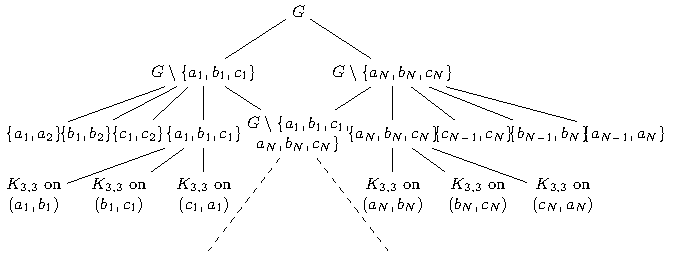
\includegraphics[height=\myMinHeight]{../../img/epsfromtikz/c2c3_of_k33s-1}
%         \caption{}\label{fig:c2c3ofk33s:b}
%     \end{subfigure}%
%     %
%     \caption{(\ref{fig:c2c3ofk33s:a}) A doublet ($C_2 \times C_3$) with each edge of the triangles replaced by a $K_{3,3}$. This pattern continues inwards for a total of $N$ triangles, indicated by the dashed lines. (\ref{fig:c2c3ofk33s:b}) Most of the DR-plan of this graph, omitting further decomposition of $K_{3,3}$ subgraphs into the separate 9 edges and of edges into the component nodes. $G\setminus\{a_i,b_i,c_i\}$ is shorthand for $G$ difference those nodes and all of the nodes in the corresponding $K_{3,3}$ subgraphs. The dashed lines indicated that this exact structure is repeated.}
%     \label{fig:c2c3ofk33s}
% \end{figure*}%

\ClearMyMinHeight
\SetMyMinHeight{.3}{../../img/svg/revised_c2c3_of_k33s}
\SetMyMinHeight{.7}{../../img/svg/revised_c2c3_of_k33s_candrp}

\begin{figure*}\centering%
    %
    \begin{subfigure}{0.3\linewidth}\centering
        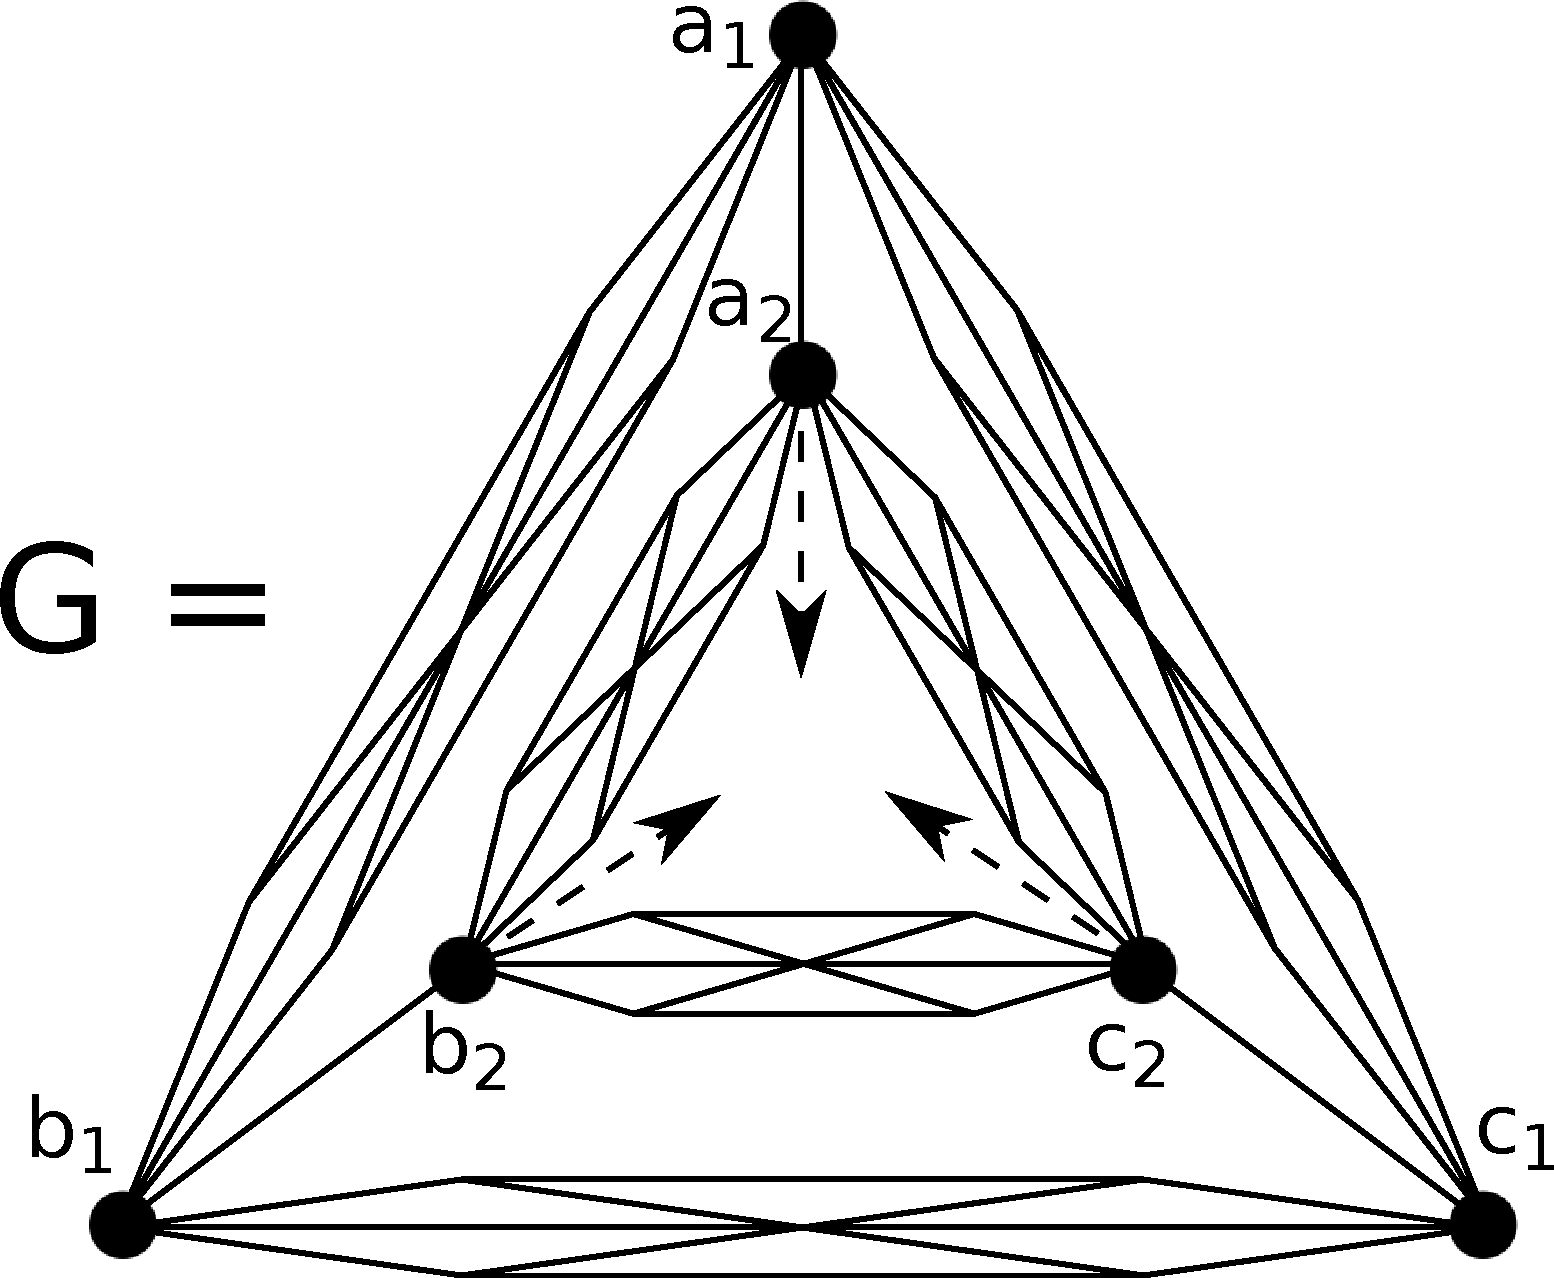
\includegraphics[height=\myMinHeight]{../../img/svg/revised_c2c3_of_k33s}
        \caption{}\label{fig:c2c3ofk33s:a}
    \end{subfigure}%
    %
    \hfill
    \begin{subfigure}{0.7\linewidth}\centering
        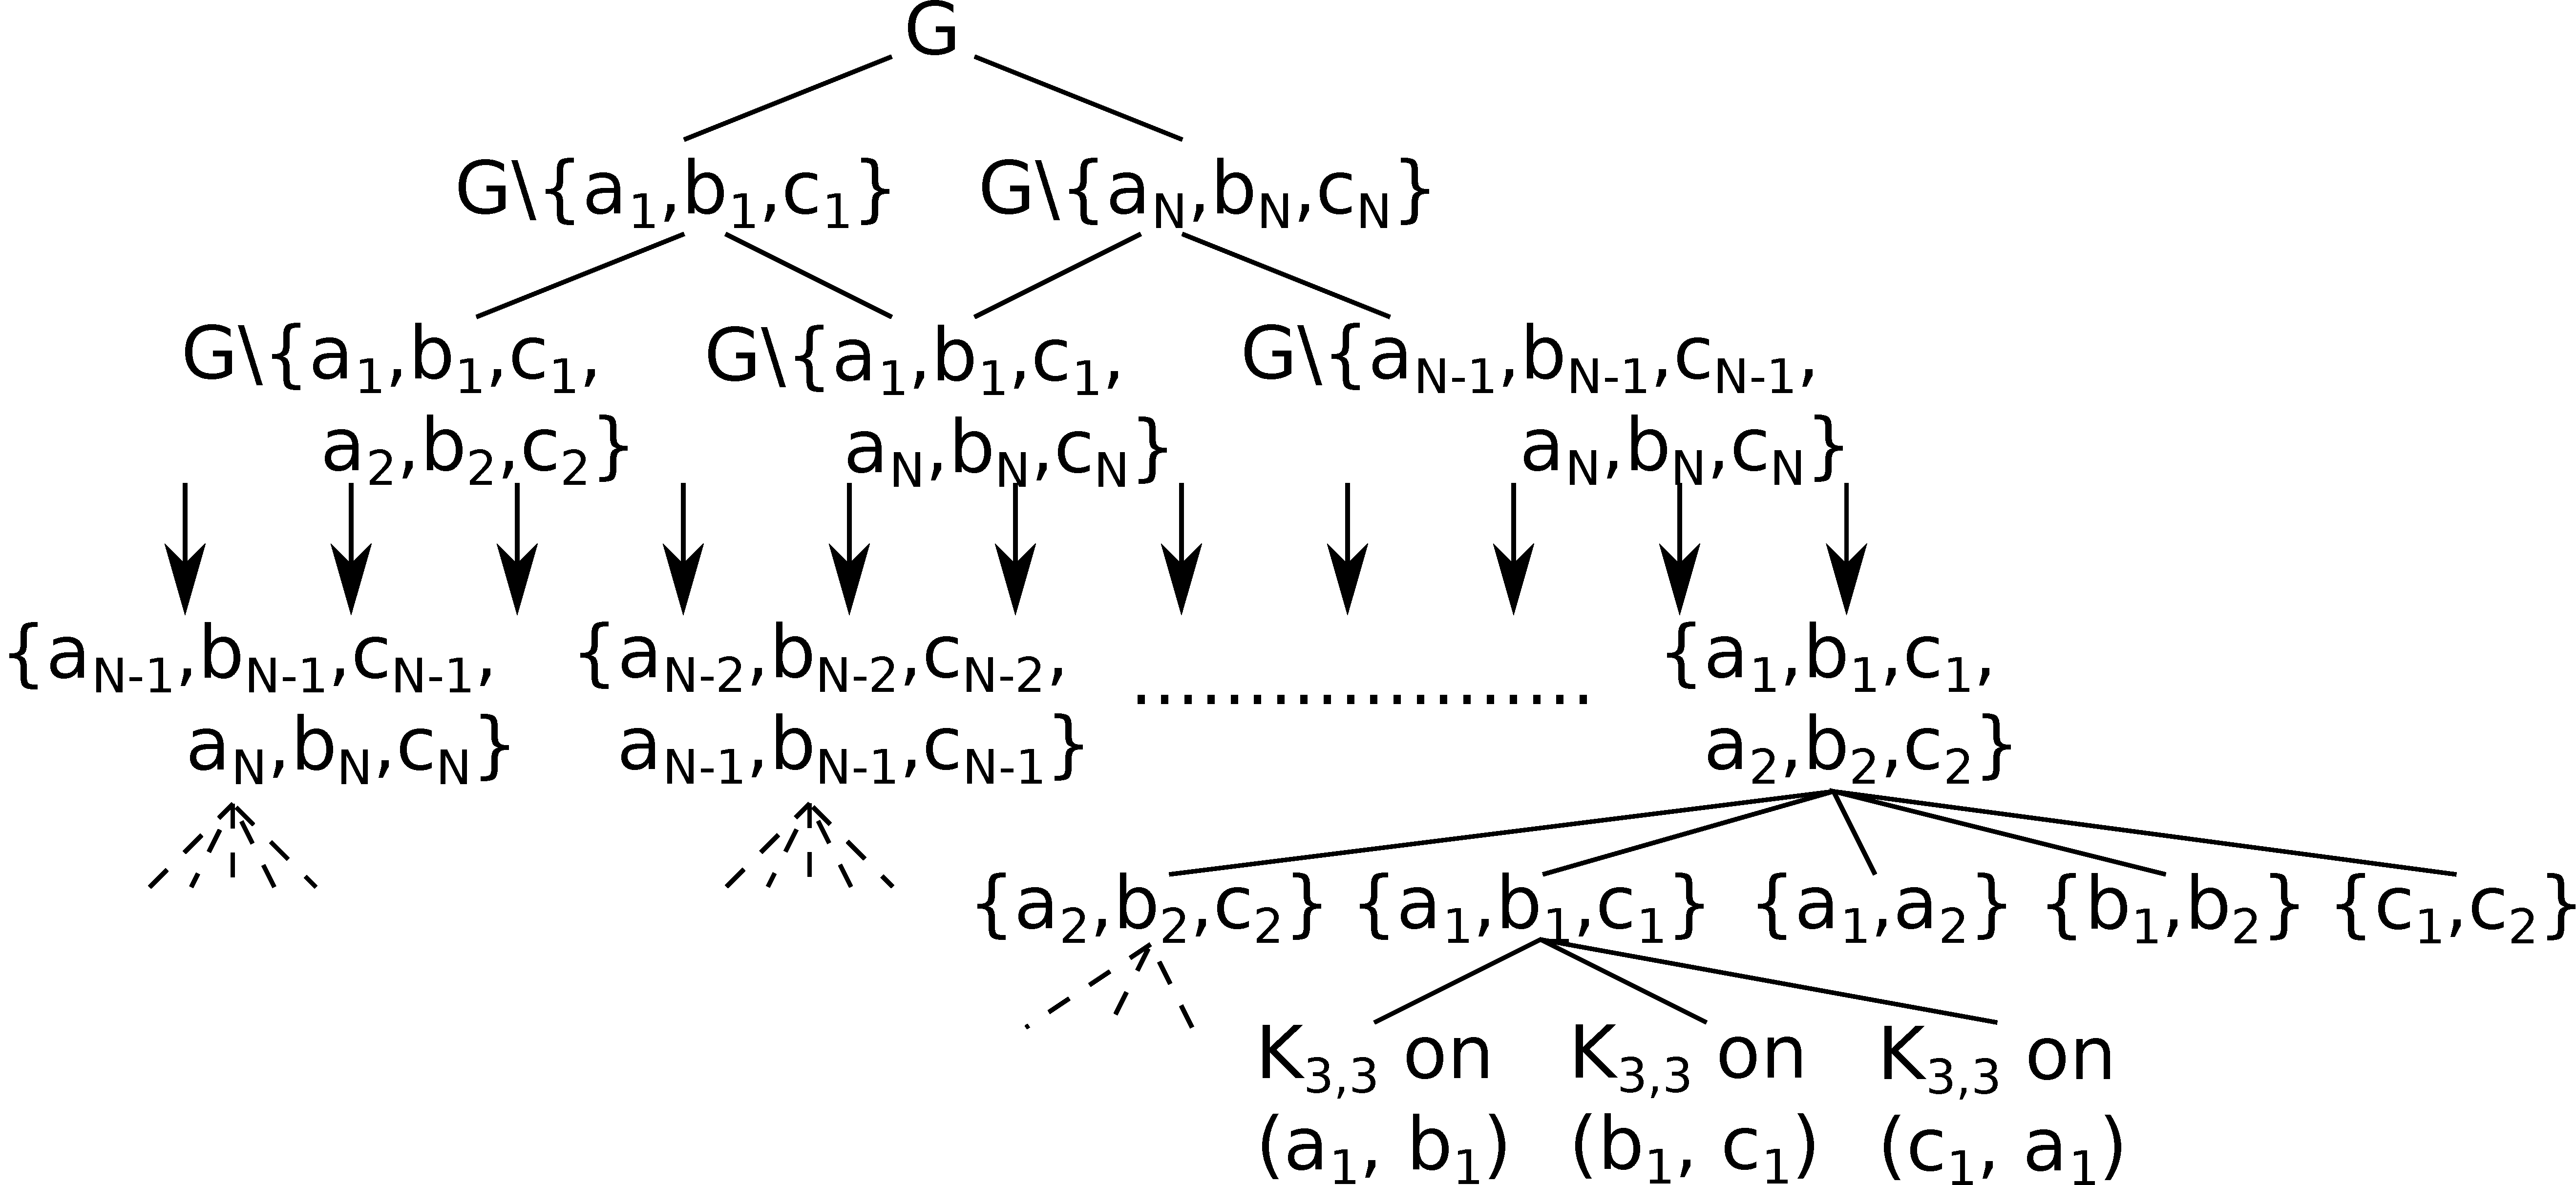
\includegraphics[height=\myMinHeight]{../../img/svg/revised_c2c3_of_k33s_candrp}
        \caption{}\label{fig:c2c3ofk33s:b}
    \end{subfigure}%
    %
    \caption{
    (\ref{fig:c2c3ofk33s:a}) A sequence of doublets ($C_2 \times C_3$) intersecting on triangles, where the edges of the triangles are replaced by $K_{3,3}$'s. This pattern continues inwards for a total of $N$ triangles, indicated by the dashed arrows. (\ref{fig:c2c3ofk33s:b}) A canonical DR-plan of $G$, drawn as a DAG. $G\setminus\{a_i,b_i,c_i\}$ is shorthand for $G$ difference those nodes and all of the nodes in the corresponding $K_{3,3}$ subgraphs. Below the third level, the obvious pattern continues until only the individual doublets are present (fourth level) with the ellipses indicating the remaining doublets between those shown. Decomposition of one of these doublets is shown. The dashed lines indicated that this exact decomposition (of the similar nodes on the level) is repeated. Further decomposition of $K_{3,3}$ subgraphs into the separate 9 edges is omitted from the figure.
    }
    \label{fig:c2c3ofk33s}
\end{figure*}%




\begin{example}
[DR-plan for self-similar structure]
    This example details the decomposition of the graph in Figure \ref{fig:c2c3ofk33s}, a canonical DR-plan of $G$. It begins with the whole (isostatic) graph as the root. The graph $G$ has only two isostatic vertex-maximal subgraphs: $G$ without the outermost triangle composed of $K_{3,3}$ graphs (triangle $1$) and $G$ without the inner triangle (triangle $N$). These intersect on $G$ without triangle $1$ and $N$ which is clearly isostatic. As explained in the proof of Theorem \ref{theorem:main}, since there are only 2 possible children, their intersection must be a node 2 levels below the parent. As expected, it is on the third level, as a child of both of $G$'s children.

    Both of $G$'s children are similar to $G$, but containing only $N-1$ triangles. Therefore, the canonical DR-plans of these children follow the same pattern. This continues downward until the individual doublets are reached (there will be multiple occurrences of the same doublets at this level, but they can be represented as the same node in a DAG).

    Further decomposition of one of these doublets is shown. The three edges between the triangles and the triangles themselves all intersect trivially pairwise. By Theorem \ref{theorem:main}, part 1, they must all be children in the DR-plan. Similarly, the triangles decompose into their three trivially intersecting $K_{3,3}$'s. Then the $K_{3,3}$ subgraphs decompose into their separate 9 edges.

    The self-similar nature of this graph is evident in the canonical DR-plan. Many structures are repeated throughout the DR-plan, allowing for shared computation in both decomposition and recombination.
\end{example}




% \subsection{Extensions}
% This framework immediately pushes through for body-pin systems via a simple reduction. If there are $N$ pins on a body, it can be represented as a 2-tree with $N$ vertices, each corresponding to a pin, making sure to select edge distances such that the distance between pins is preserved. E.g.\ a body with two pins is an edge, three pins is a triangle, etc. Any bodies that share a pin now intersect on their vertex that corresponds to that pin. Now we have a bar-joint representation of the body-pin system in 2D and all proofs follow.

% With more effort, it can be shown that pinned line-incidence systems can also use this framework. This is done in section \ref{XXX}.


\subsection{Algorithm}
\label{sec:DRP:algo}

The algorithm for finding an optimal DR-plan relies on key structural properties of canonical DR-plans that are revealed by the proof of Theorem~\ref{theorem:canonical_exists_and_is_optimal}. We list these properties before describing the algorithm. Furthermore, in order to deal with the apparent non-uniqueness of a canonical DR-plan (in the case when the children of a node have non-trivial intersections), and to make the canonical DR-plan more malleable for algorithmic purposes, we define a key notion of a \dfn{sequential DR-plan} that is obtained from a canonical DR-plan, and also turns out to be an optimal DR-plan. A sequential DR-plan further clarifies the essential uniqueness of canonical DR-plans. First, we present a recursive definition of the canonical DR-plan, which is more useful in this section, and make an important observation.

\begin{definition}
[Canonical DR-plan]
\label{def:canonical_drp_rec}
    A \dfn{canonical DR-plan} of $G$ is recursively defined as follows:
    \begin{enumerate}
        \item Base case: When $G$ is a single edge, the canonical DR-plan for $G$ is $G$ itself.
        \item In case the pairwise intersections of the proper vertex-maximal rigid subgraphs $C_i$ of $G$  are all trivial, take the children of $G$ to be the roots of the canonical DR-plans for $C_i$.
        \item In case there are two proper vertex-maximal rigid subgraphs $C_i$ and $C_j$ of $G$ with non-trivial intersection, take the children of $G$ to be the roots of the canonical DR-plans for $C_i$ and $C_j$.
    \end{enumerate}
    % When $G$ is a single edge (base case), the canonical DR-plan for $G$ is $G$ itself.
\end{definition}
\todo{What if input is not isostatic? What roots?}

\begin{observation}
[Canonical DR-plan size]
    While all canonical DR-plans of independent graphs are optimal, based on the choice of children in Case (3) above they can have varying \dfn{size} (i.e.\ the number of unique nodes). If we want the canonical DR-plan to have small size (linear \todo{or just polynomial?} in the number of vertices) we can choose the children in the following fashion: In Case (3) above, a canonical DR-plan for $C_i$ (resp.\ $C_j$) is further recursively defined by taking the children of $C_i$ (resp.\ $C_j$) to be the roots of a canonical DR-plan of $C_i\cap C_j$ (which is rigid, by Lemma~\ref{lemma:combined_lemma}), and a canonical DR-plan of $C_i\setminus C_j$ (resp. $C_j\setminus C_i$) (which are not rigid, by Observation~\ref{lemma:union_intersection} and Lemma~\ref{lemma:combined_lemma}).

    Note that a canonical DR-plan can have more than one node representing the same rigid subgraph if and only if Case (3) occurs.
\end{observation}


% Observation XX[recursive definition of canonical DR-plan]:
% \begin{observation}
    % In a canonical DR-plan of an independent graph, the portion of the DR-plan rooted at any node $C_i$ is a canonical DR-plan for $C_i$. \todo{unneccessary sentence.}

    % In other words, a canonical DR-plan of $C$ is recursively defined by taking the children of $C$ to be the roots of canonical DR-plans for (a) each proper vertex-maximal rigid  subgraph of $C$, in case their pairwise intersection is trivial or (b) two proper vertex-maximal rigid  subgraphs $C_i$ and $C_j$ of $C$, in case their intersection is non-trivial. When $C$ is trivial (base case), the DR-plan for $C$ is $C$ itself.
    % \todo{delete everything above, move definition 6 here.}

    % In the latter Case (b) above, a canonical DR-plan for $C_i$ (resp.\ $C_j$) is further recursively defined by taking the children of $C_i$ (resp.\ $C_j$) to be the roots of a canonical DR-plan of $C_i\cap C_j$ (which is rigid, by Lemma~\ref{lemma:combined_lemma}), and a canonical DR-plan of $C_i\setminus C_j$ (resp. $C_j\setminus C_i$) (which are not rigid, by Observation~\ref{lemma:union_intersection} and Lemma~\ref{lemma:combined_lemma}).

    % Note:
    % a canonical DR-plan has more than one node representing the same rigid subgraph if and only if Case (b) occurs.
% \end{observation}


Now we define the sequential DR-plan in a manner analogous to Definition~\ref{def:canonical_drp_rec}.

\begin{definition}
[(Pseudo-)Sequential DR-plan, appendage, partner, core]
\label{def:seqdrp}
    A \dfn{pseudo-sequential DR-plan} of $G$ is recursively defined as follows:
    \begin{enumerate}
        \item Base case: When $G$ is an edge, the sequential DR-plan for $G$ is $G$ itself.
        \item In case the pairwise intersections of the proper vertex-maximal rigid subgraphs $C_i$ of $G$  are all trivial, take the children of $G$ to be the roots of the sequential DR-plans for $C_i$.
        \item In case there are two proper vertex-maximal rigid subgraphs $C_i$ and $C_j$ of $G$ with non-trivial intersection, take the children of $G$ to be the roots of sequential DR-plans for $C_j\setminus C_i$ (called an \dfn{appendage}), and $C_i$ (called its \dfn{partner}).
        % If the decomposition of the partner $C_i$ results in Case (2), one of the children will be $C_i\cap C_j$, which we call the \dfn{core}.\footnote{Which can be thought of as partner to appendage $C_i\setminus C_j$.}\todo{Is this okay? I don't know how to say this succinctly.}
    \end{enumerate}

    % DR-plans satisfying Requirements 1,2, and 3 are called \dfn{pseudo-sequential.}

    \dfn{Sequential DR-plans} must satisfy another requirement:

    \begin{enumerate}
        \setcounter{enumi}{3}
        \item Let $C$ be a node and $C_s$ the set of its siblings in a sequential DR-plan. If there is a descendant $D$ of $C$, with siblings $D_s$  possessing the property that $C\cup C_s\setminus D_s$ is rigid, then for the contiguous sequence of nodes $D'$ on the path from $C$ to $D$, we require that $C\cup C_s \setminus D'_s$ be rigid, where $D'_s$ is the set of siblings of $D'$. Here $C$, $D$ and $D'$ are the partners of the appendages $C_s$, $D_s$ and $D'_s$.
        %
    \end{enumerate}

    When the graph is independent and the DR-plan is sequential (Property (4) holds), if the parent of $C\cup C_s$ falls under Property (2), while $C\cup C_s$ falls under Property (3), then the lowest descendant $D$ as above is called the \dfn{core} of $C\cup C_s$.
\end{definition}

\begin{figure}\centering
    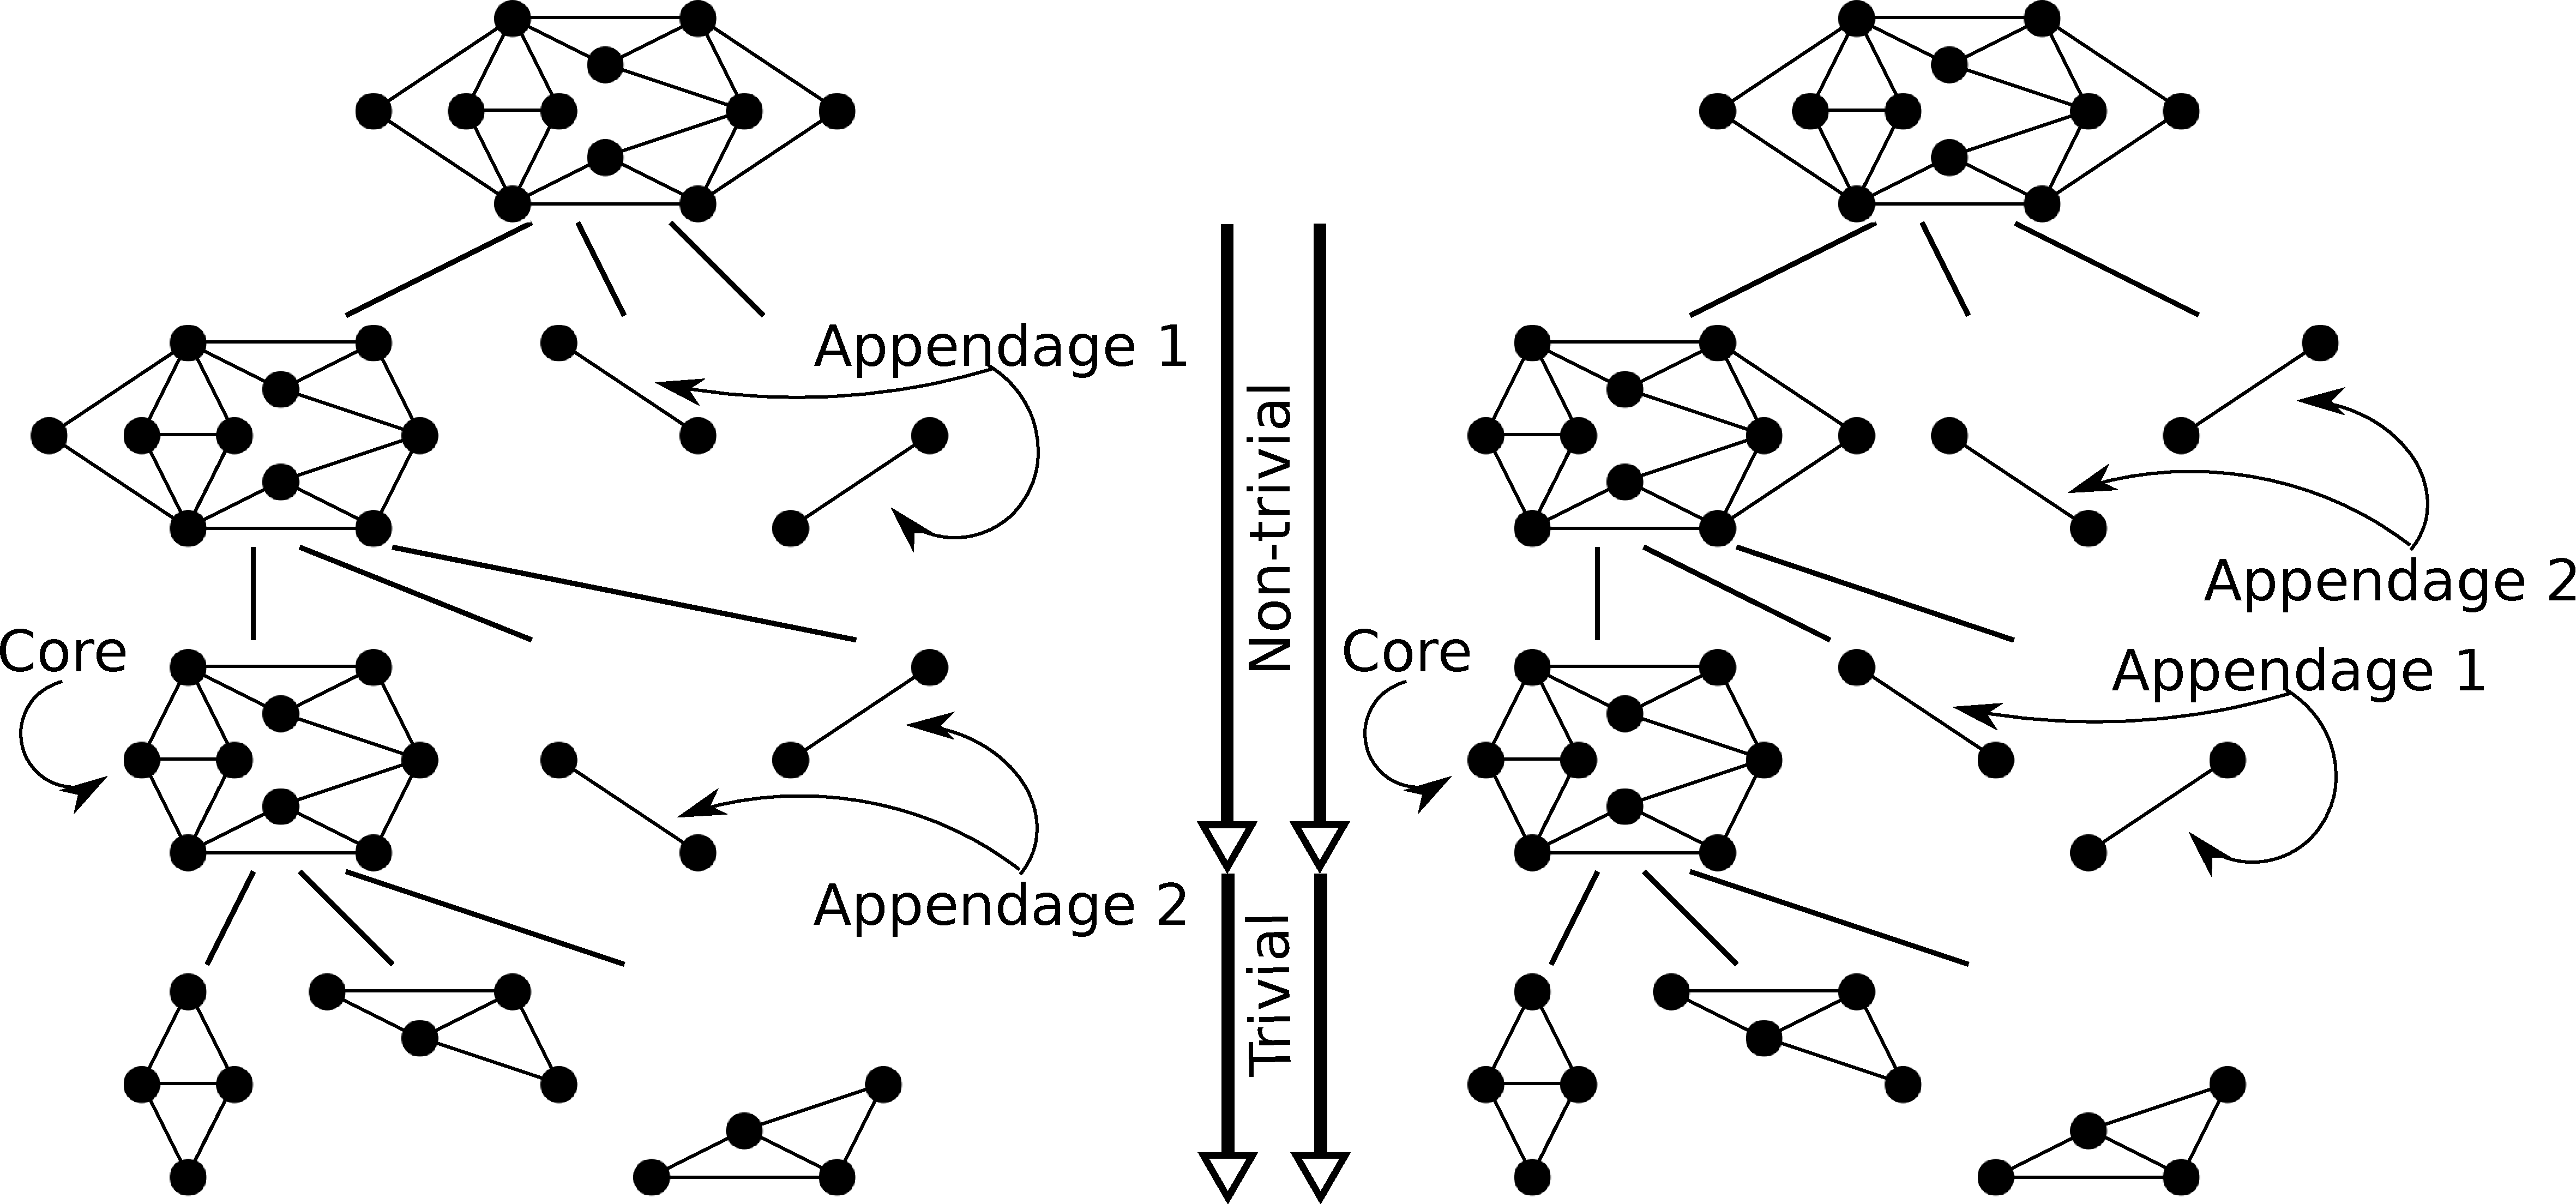
\includegraphics[width=\linewidth]{../../img/svg/drp_triv_and_non}
    \caption{Two sequential DR-plans of the same isostatic input graph. \todo{More caption.}}
    \label{fig:seqdrp_nonuniqueness}
\end{figure}


\begin{remark}
[Essential uniqueness of sequential DR-plans]
\label{remark:seq_is_essentially_unique}
    For sequential DR-plans of independent graphs, Property (3) of the above definition appears asymmetric with respect to $i$ and $j$; but in fact, $i$ and $j$ can be switched, using the appendage $C_i\setminus C_j$ instead. Let $C_1, C_2, \ldots, C_N$ be a complete list of proper vertex-maximal rigid subgraphs of $C$. Their pairwise intersections must all be nontrivial, and their common intersection, called a \dfn{core}, is isostatic by Lemma~\ref{lemma:combined_lemma}. Denote by $A_i$ the $i^\text{th}$ appendage, where $A_i = C_j\setminus C_i$, for any $j\neq i$. Note that $C_i = C\setminus A_i$; and $C_i = \bigcap_i{C_i} \bigcup_{j\ne i}{A_j}$. Choosing a particular ordering of the $C_i$, i.e.\ choosing the maximal rigid components of a particular appendage, say $A_1$, and its partner $C_1$ to be the children of $C$ simply pushes down the nodes corresponding to the appendages $A_2, A_3, \ldots, A_N$ to a lower level of the sequential DR-plan and the corresponding partners are created as $C_1\cap C_2, C_1\cap C_2\cap C_3, \ldots$; the last appendage, $A_N$, will always have the core, $\bigcap_i{C_i}$, as its partner. Thus, modulo the ordering of appendages, the sequential DR-plan is in fact unique. See Figure~\ref{fig:seqdrp_nonuniqueness}.

    Furthermore, any rigid subgraph appears in at most one node of a sequential DR-plan. Also, if an edge $e$ of $G$ belongs in the rigid subgraph at any two nodes $A$ and $B$ of a sequential DR-plan, then either $A\subset B$ or $B\subset A$. Since the leaves of sequential DR-plan tree are the $O(|V(G)|)$ edges of the independent input graph, this implies the size of the tree is $O(|V(G)|)$.
\end{remark}


\begin{lemma}
[Pseudo-sequential to sequential DR-plan]
    Any pseudo-sequential DR-plan for an independent graph can be converted to a sequential DR-plan (satisfying Property (4)) in time $O(|V(G)|)$.
\end{lemma}

\begin{proof}
    For independent graphs, note that Property (2) and (3) of Definition~\ref{def:seqdrp} automatically imply that the following holds for a pseudo-sequential DR-plan: for a node $G$ that falls under Property (2), there is no child $C$ of $G = C\cup C_s$ for which there is a descendant $D$ with siblings $D_s$ possessing the property that $C\cup C_s \setminus D_s$ is rigid; for a node $G$ that falls under Property (3), such a descendant $D$ exists for a unique child $C$ of the node $G=C\cup C_s$, as well as for unique children of all $D'$ on the path from $C$ to $D$. Furthermore, for all such $D'$, it automatically holds that $D'\cup D'_s \setminus D_s$ is rigid. We call this \emph{Property (4')} (since it is a parallel property of Property (4) of Definition~\ref{def:seqdrp}).

    Given a pseudo-sequential DR-plan of an independent graph where nodes with Property (3) of Definition~\ref{def:seqdrp} are labeled, we show how to enforce Property (4) of Definition~\ref{def:seqdrp}, for a node $C\cup C_s$ with Property (3), i.e.\ when there is a descendant $D$ with siblings $D_s$ possessing the property that $C\setminus D_s \cup C_s$ is rigid.

    Let $D$ be any such descendant where Property (4) does not hold and let $D^*$ (with siblings $D^*_s$) be the highest node along the path from $C$ to $D$ where $C\cup C_s \setminus D^*_s$ is not rigid.
    Since we know that $C\cup C_s \setminus D_s$ is in fact rigid by the hypothesis of Property (4), and since Property (4') holds for $D^*$, i.e.\ $D^*\cup D^*_s \setminus D_s$, we ``switch $D^*_s$ with $D_s$'' by setting up the partners and appendages along the path from $D^*$ to $D$ as follows.

    % At the level of the node $D^*$, the appendage is $D_s$ and the partner is $D^*\cup  D^*_s \setminus D_s$ (which we know to be rigid by Property (4)); At the level of each node $D'$ on the path starting from a child of $D^*$ down to $D$, the appendage is parent$(D')_s$ \todo{Is this correct? Or is it just $D'_s$?} and its partner is $D'\cup D'_s\setminus D_s$ (which we know to be rigid by Property (4')).
    At the level of each partner node $D'$ on the path starting from $D$ to a child of $D^*$ the appendage becomes parent$(D')_s$ and the new partner becomes $D'\cup D'_s\setminus D_s$ (which we know to be rigid by Property (4')). In particular, at the level of the partner node $D$ the appendage becomes parent$(D)_s$ and the new partner remains $D$. However, at the next higher level the old partner node parent$(D) = D\cup D_s$ becomes the new partner $D\cup$ parent$(D)_s$ of the new appendage is parent$($parent$(D))_s$.

    At the level of the node $D^*$, the appendage becomes $D_s$ and the partner becomes $D^*\cup D^*_s\setminus D_s$ (which we know to be rigid by Property (4)).

    Once the above switch has been completed, moving $D_s$ up the path from $D$ to $C$,
    % Once the above switch has been completed, moving $D_s$ up the path from $C$ to $D$,
    it is unnecessary to inspect any of the siblings of any of the nodes along this path. This is because $C$ is the unique child of $C\cup C_s$ for which such a descendant $D$ even exists, and the same uniqueness holds for every node that is on the path from $C$ to $D$.

    Note that in the same iteration, the algorithm can simultaneously perform the above process on all such descendants of $C$ for which Property (4) does not hold, since they must all be on the same descending path from $C$. Once Property (4) has been enforced for all such descendants of $C$, the algorithm has found the core for $C\cup C_s$, namely the last node in a contiguous path of nodes $D'$ starting down from $C$, for which $C\cup C_s\setminus D'_s$ is rigid. The order of appendages of all of these nodes are interchangeable (with appropriate partners) as indicated in Remark~\ref{remark:seq_is_essentially_unique}.

    The algorithm then proceeds to the next node $C\cup C_s$ with Property (3), for which there is a descendant $D$ with siblings $D_s$ possessing the property that $C\setminus D_s \cup C_s$ is rigid and for which Property (4) does not hold.

    This process continues until Property (4) always holds, resulting in a sequential DR-plan. It is clear that the algorithm visits any given node of the sequential DR-plan at most $O(1)$ times resulting in a linear time complexity.

    The next observations follow from the abovementioned structure of a sequential DR-plan and from the proof of Theorem~\ref{theorem:canonical_exists_and_is_optimal}.
\end{proof}

% \begin{observation}
% [Sequential-canonical]
%     A sequential DR-plan for an independent graph $G$ can be converted to a canonical DR-plan in time linear in the number of its nodes, which is $O(|V(G)|)$. \todo{This isn't true... in O(nodes) of which plan?... there could be $n^2$ nodes in the canonical...}
% \end{observation}

\begin{observation}
[Sequential is optimal]
    A \todo{psuedo-}sequential DR-plan of an independent graph is optimal.
    \todo{(Psuedo-)sequential DR-plans of independent graphs are optimal.}
\end{observation}

\begin{proof}
    We need to show the statement:
    (*) the max fan-in (i.e.\ number of children) of any sequential DR-plan for an independent graph $G$ is no larger that of some canonical DR-plan for $G$. By Theorem~\ref{theorem:canonical_is_optimal}, this would imply that the sequential DR-plan is optimal.

    Recall that both sequential and canonical DR-plans are defined recursively. We will prove the statement (*) by induction on the height of a sequential DR-plan for $G$. Induction hypothesis: (*) holds for independent graphs $G$ with sequential DR-plans of height $h$. Induction step: a sequential DR-plan of height $h+1$ rooted at a node $G$ consists of sequential DR-plans (of height at most $h$) rooted at its children $C$.
    The base case (height of 0, i.e.\ single edges) trivially holds.

    It is sufficient to show (a) the children $C$ will exist somewhere in some canonical DR-plan, and (b) $|C|$ is less than or equal to the max fan-in of some canonical DR-plan. Given (a), then by the recursive definition of canonical DR-plans, these nodes are the roots of canonical DR-plans, thus the induction hypothesis applies to the nodes in $C$. Additionally given (b), the proof of the induction step of (*) is complete.

    Case (1):
    When the isostatic vertex-maximal proper subgraphs of $G$ have trivial intersections, the children of $G$ in any canonical DR-plan are the same set $C$ of children in any sequential DR-plan. Thus both conditions (a) and (b) are immediately satisfied.

    Case (2):
    When the isostatic vertex-maximal proper subgraphs of $G$ have non-trivial intersections, the children $C$ are the isostatic components of some appendage, $A_i$, and its partner. The partner will be a child of $G$ in some canonical DR-plan. Furthermore, in any canonical DR-plan there will be some node $N-1$ levels below $G$ (where $N$ is the number of appendages) containing the core plus appendage $A_i$. In some canonical DR-plan, the children of this node will be the components of $A_i$ and the core. This node has the same fan-in as $G$ in the sequential DR-plan, satisfying (b), and, along with the partner (a child of $G$), shows that some canonical DR-plan has all the nodes in $C$, thereby satisfying (a).
\end{proof}

% \begin{proof}
%     Any sequential DR-plan, $\seqdrpx{G}$, has maximum fan-in no greater than that of some canonical DR-plan, $\candrpx{G}$, of the same independent graph $G$. By Theorem~\ref{theorem:canonical_is_optimal}, this implies a sequential DR-plan is also optimal. Consider node $C$ that appears in both $\seqdrpx{G}$ and $\candrpx{G}$ with isostatic vertex-maximal proper subgraphs (clusters) $C_1, C_2, \ldots, C_N$.
%     We prove this recursively by showing that node $C$ in $\seqdrpx{G}$ and any descendant of $C$ that is not in $\candrpx{G}$ has fan-in less than or equal to the maximum fan-in of $\candrpx{G}$.

%     Case 1: If the clusters of $C$ have pairwise trivial intersections, then node $C$ has the same set of children and fan-in in both $\seqdrpx{G}$ and $\candrpx{G}$.

%     Case 2: Otherwise, the clusters of $C$ have pairwise non-trivial intersection, and we call the common intersection the core. The children of node $C$ in $\seqdrpx{G}$ will be the components of the appendage, $A_1$, and its partner, $T_1$. In $\candrpx{G}$, there will be some node $D$ that is $A_1$ union the core; $D$ can have clusters with either trivial or non-trivial intersections.

%     Case 2a: In the trivial case, node $D$ decomposes into the core and the components of $A_1$; thus, the fan-in of node $C$ in $\seqdrpx{G}$ is equal to the fan-in of $D$ in $\candrpx{G}$ and they both have the components of $A_1$ as children, leaving $T_1$ to be shown to be optimally decomposed in $\seqdrpx{G}$.

%     Case 2b: In the non-trivial case, there is some new core of $D$, so there will be some node $D'$ in $\candrpx{G}$ that is $A_1$ union the core of $D$; this pattern will continue until we eventually find $D^*$ with clusters that intersect trivially. Similar to Case (2b), the fan-in of node $C$ in $\seqdrpx{G}$ is equal to the fan-in of $D^*$ in $\candrpx{G}$ and they both have the components of $A_1$ as children, leaving $T_1$ to be shown to be optimally decomposed in $\seqdrpx{G}$.

%     The decomposition of $T_1$ in $\seqdrpx{G}$ will be the components of appendage $A_2$ and its partner $T_2$. Similarly, $\candrpx{G}$ will contain core union $A_2$, and so we must now show $T_3$ is decomposed optimally in a sequential DR-plan. This continues to the node containing $T_{N-1}$, the core union appendage $A_N$, in $\seqdrpx{G}$, which we know to be a node in $\candrpx{G}$.
% \end{proof}


\begin{definition}
[\Branch]
    Given a sequential DR-plan $P_G$ for an isostatic graph $G$, and an edge $e \in G$, the \branchGePG\ is the subtree of the DR-plan consisting of the path from the leaf containing $e$ to the root containing $G$, together with the children of all the nodes on this path, which are the leaves of \branchGePG.
\end{definition}

\begin{observation}
[Sequential DR-plan recursively from \branches]
\label{obs:seqplan_rec_from_branches}
    A sequential DR-plan $P_G$ for an isostatic graph $G$ is obtained from \branchGePG\ by recursively attaching to each of its leaves $L$ a sequential DR-plan $P_L$ for $L$.
\end{observation}

The next two Lemmas are the crux of our $O(|V|^3)$ algorithm to find a sequential DR-plan.

\begin{lemma}
[\Branch\ leaves from components]
    Let $G$ be isostatic, $e$ be an edge in $G$, and $\componentsx{G\setminus e}$ be the set of maximal rigid components of $G\setminus e$. Then there is a sequential DR-plan $P_G$ for $G$ such that $\componentsx{G\setminus e}$ is exactly the set of leaves of \branchGePG\ (minus $e$ itself).
\end{lemma}

\begin{proof}
    Follows from the structure of a sequential DR-plan and the definition of \branchGePG.
\end{proof}



\ClearMyMinHeight
\SetMyMinHeight{0.240}{../../img/svg/seq_proof_figs_a}
\SetMyMinHeight{0.24}{../../img/svg/seq_proof_figs_b}
\SetMyMinHeight{0.240}{../../img/svg/seq_proof_figs_c}
\SetMyMinHeight{0.24}{../../img/svg/seq_proof_figs_d}

\begin{figure*}\centering%
    % \begin{subfigure}[t]{0.27\linewidth}
    %     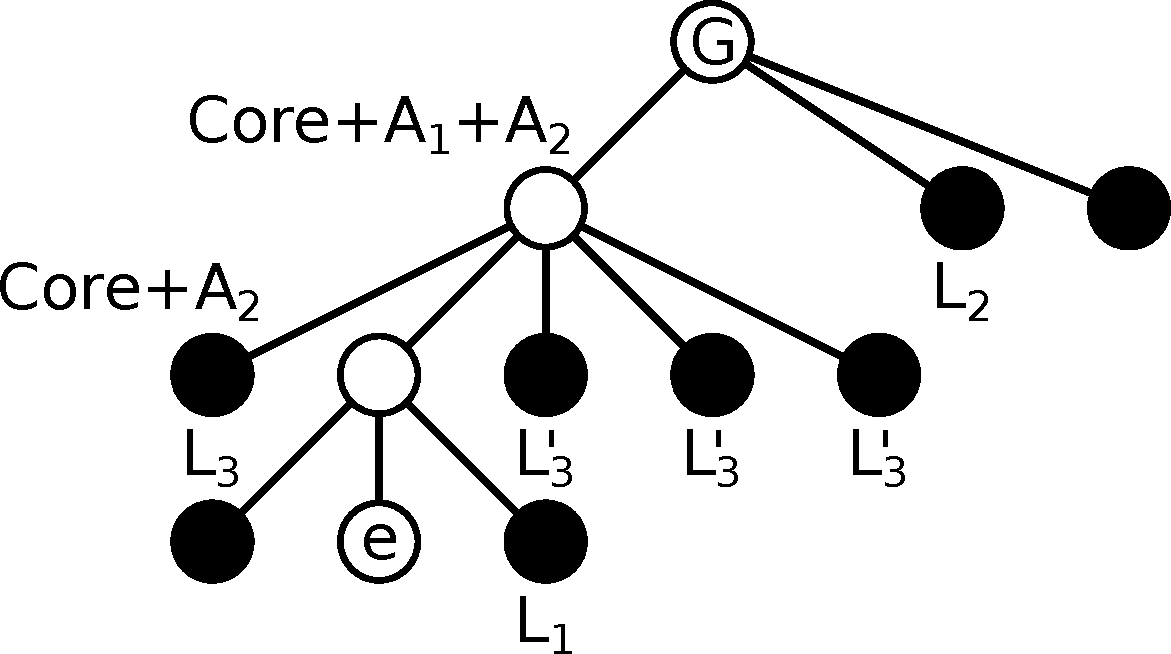
\includegraphics[width=\linewidth]{../../img/svg/seq_proof_figs_a}
    %     \caption{}\label{fig:seq_proof:a}
    % \end{subfigure}%
    % %
    % \hfill
    % \begin{subfigure}[t]{0.17\linewidth}
    %     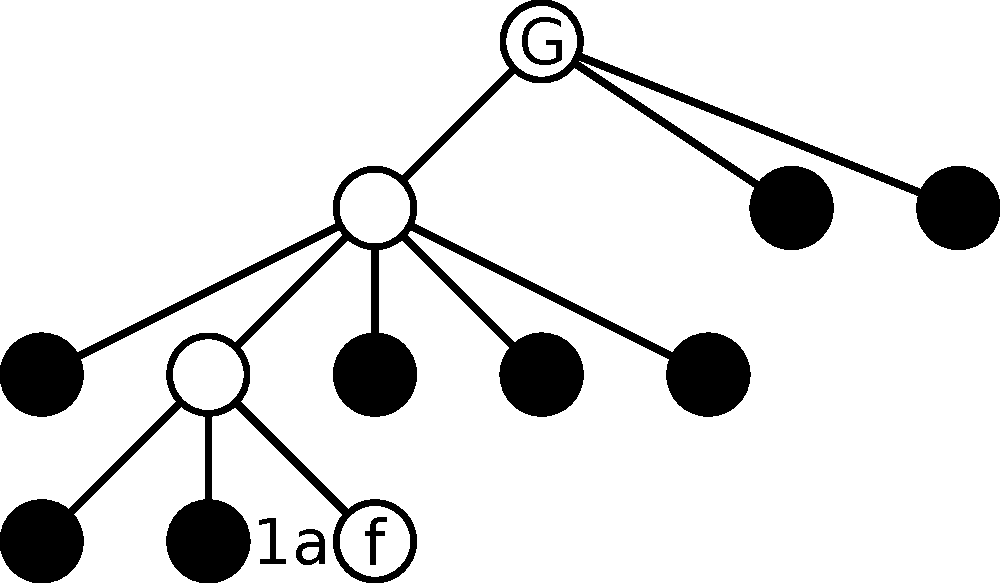
\includegraphics[width=\linewidth]{../../img/svg/seq_proof_figs_b}
    %     \caption{}\label{fig:seq_proof:b}
    % \end{subfigure}%
    % %
    % \hfill
    % \begin{subfigure}[t]{0.25\linewidth}
    %     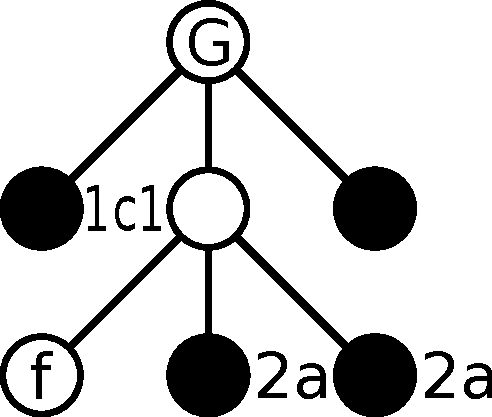
\includegraphics[width=\linewidth]{../../img/svg/seq_proof_figs_c}
    %     \caption{}\label{fig:seq_proof:c}
    % \end{subfigure}%
    % %
    % \hfill
    % \begin{subfigure}[t]{0.23\linewidth}
    %     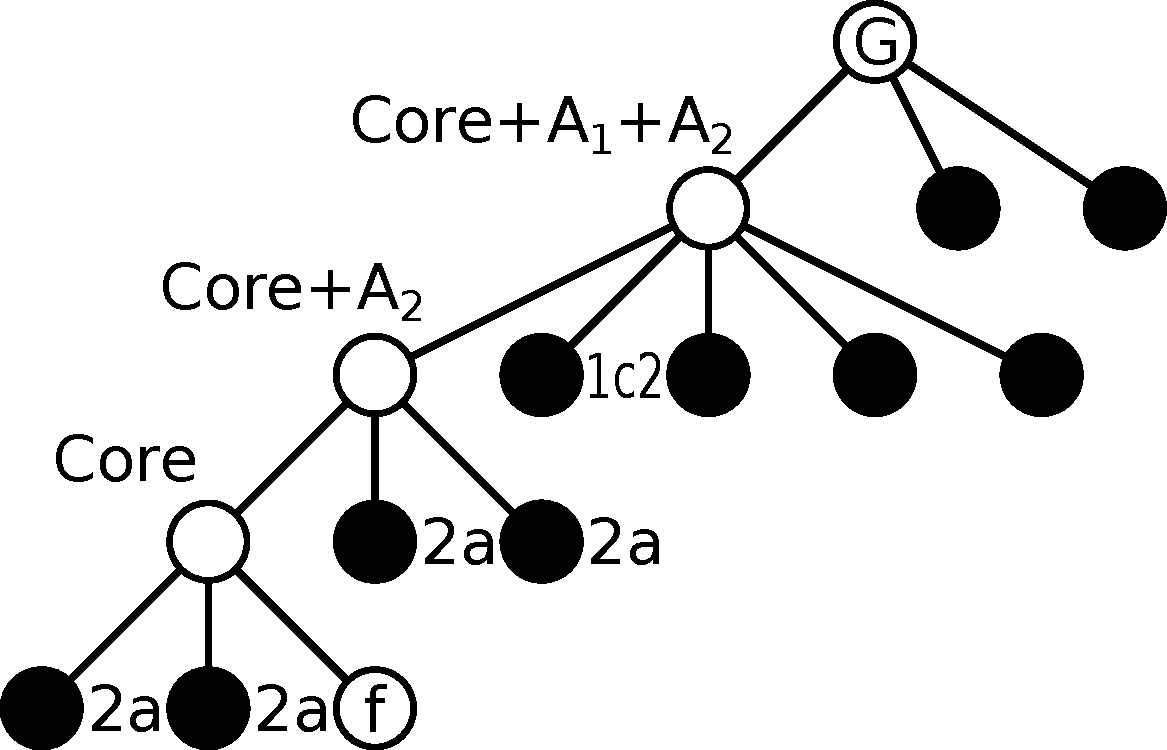
\includegraphics[width=\linewidth]{../../img/svg/seq_proof_figs_d}
    %     \caption{}\label{fig:seq_proof:d}
    % \end{subfigure}%
    \begin{subfigure}{0.240\linewidth}\centering
        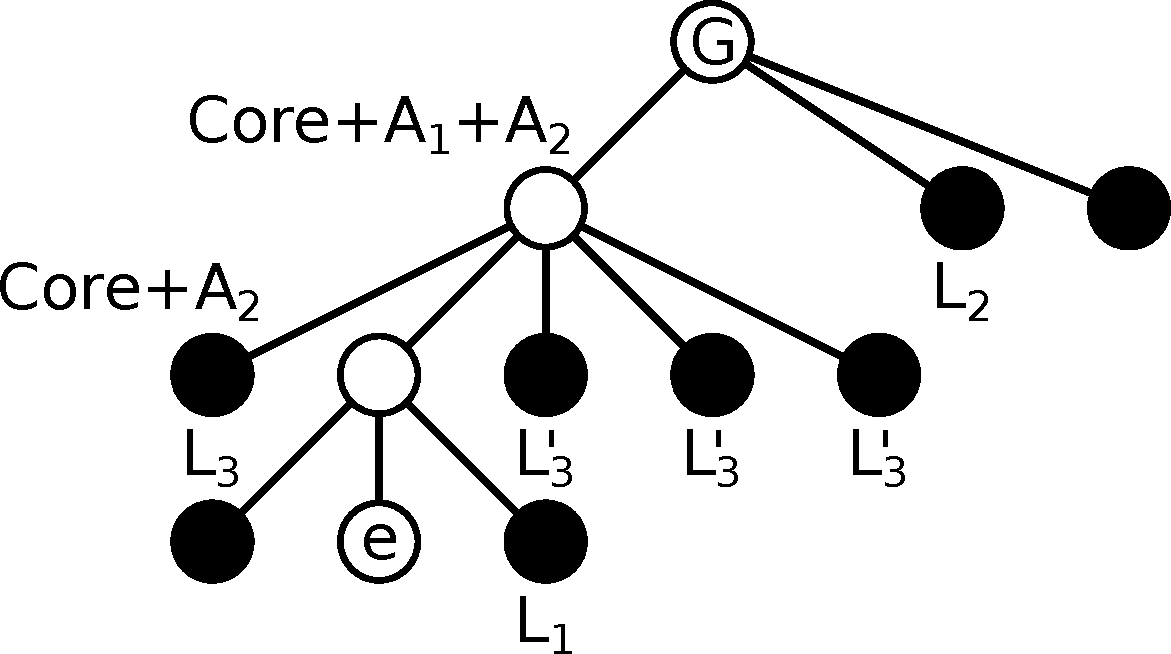
\includegraphics[height=\myMinHeight]{../../img/svg/seq_proof_figs_a}
        \caption{}\label{fig:seq_proof:a}
    \end{subfigure}%
    %
    \hfill
    \begin{subfigure}{0.24\linewidth}\centering
        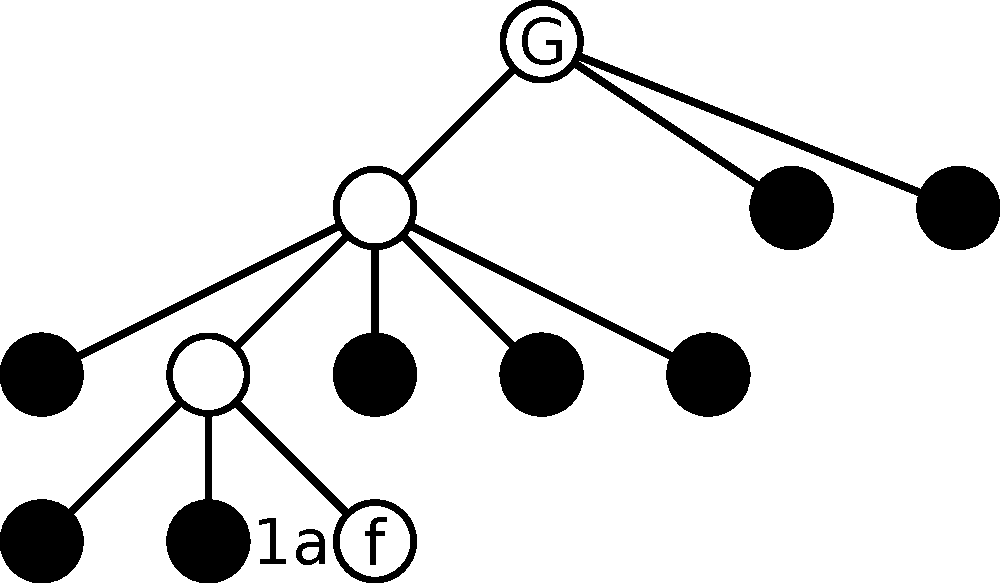
\includegraphics[height=\myMinHeight]{../../img/svg/seq_proof_figs_b}
        \caption{}\label{fig:seq_proof:b}
    \end{subfigure}%
    %
    \begin{subfigure}{0.240\linewidth}\centering
        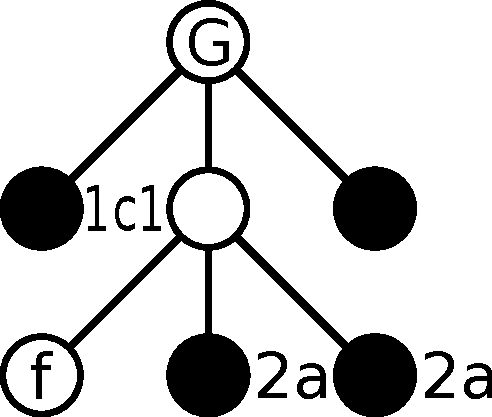
\includegraphics[height=\myMinHeight]{../../img/svg/seq_proof_figs_c}
        \caption{}\label{fig:seq_proof:c}
    \end{subfigure}%
    %
    \hfill
    \begin{subfigure}{0.24\linewidth}\centering
        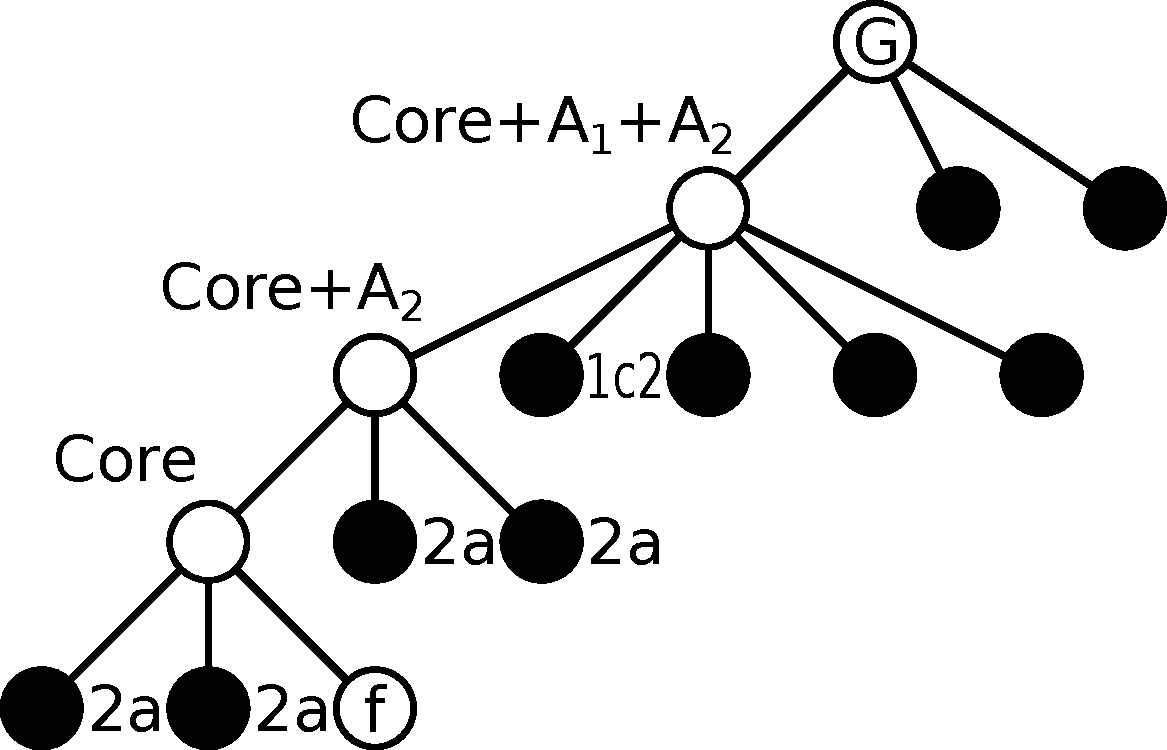
\includegraphics[height=\myMinHeight]{../../img/svg/seq_proof_figs_d}
        \caption{}\label{fig:seq_proof:d}
    \end{subfigure}%

    \caption{
    Figure (\ref{fig:seq_proof:a}) depicts $\branchx{G,e,P_G}$, the black nodes are the $\componentsx{G\setminus e}$. The node labeled `Core+A$_1$+A$_2$' is a subgraph of $G$ that has 2 isostatic vertex-maximal proper subgraphs intersecting non-trivially.
    %
    Figure (\ref{fig:seq_proof:b}) depicts $\branchx{G,f,P_G}$ of the edge labeled $f\in L_2$ (from Figure (\ref{fig:seq_proof:a})). Similarly, the black nodes are the $\componentsx{G\setminus f}$. These leaves are labeled with the cases discussed in the proof of Lemma~\ref{lem:branch-from-branch-leaves}.
    %
    Figure (\ref{fig:seq_proof:c}) depicts $\branchx{G,f,P_G}$ of the edge labeled $f$ in the core in $L_1$ (from Figure (\ref{fig:seq_proof:a})). Note that based on the choice of $e$ as the first edge, we get a sequential DR-plan that looks like Figure (\ref{fig:seq_proof:c}), if we had chosen an edge from appendage A$_2$ the second and third level would be flipped.
    %
    Figure (\ref{fig:seq_proof:d}) depicts $\branchx{G,f,P_G}$ of the edge labeled $f$ in the appendage A$_1$ in $L_1$ (from Figure (\ref{fig:seq_proof:a})). Note that this contains a node $D$ that has Case 3. With this $D$, $D\cup L_1$ is `Core+A$_1$+A$_2$' and $D\cap L_1$ is `Core'. The leaves labeled L$_1'$ in Figure (\ref{fig:seq_proof:a}) are the leaves that will allow us to find the node on the path from $G$ to $e$ that is their sibling (the parent of $e$).
    %
    % Take edge $a\in G$, the $\componentsx{G\setminus a}$ is the set of nodes marked with an `x' in figure xx. The entire figure shows $\branchx{G,a,P_G}$, where $P_G$ is the sequential DR-plan of $G$, however, we do not yet know the contents of the `circle' nodes or the order of the nodes in the \branch.
    %
    % So we take leaf $L$ (an element of $\componentsx{G\setminus a}$) and edge $b\in L$, and find $\components{G\setminus b}$. The this set is the leaves of the $\branchx{G,b,P_G}$, shown in figure xx.
    }
    \label{fig:seq_proof}
\end{figure*}


\begin{lemma}
[\Branch\ from \branch\ leaves]
\label{lem:branch-from-branch-leaves}
    For an isostatic graph $G$ containing an edge $e$, the \branchGePG\ for a sequential DR-plan $P_G$ can be constructed from $\componentsx{G\setminus e}$, i.e.\ from the set of leaves of \branchGePG, by carrying out---for each leaf $L$---one computation of $\componentsx{G\setminus f}$, where $f$ is any edge in $L$.
\end{lemma}

\begin{proof}
    First note that in order to obtain \branchGePG\ from the set of subgraphs at its leaves, it is sufficient to find the subgraphs at the nodes along the path from $e$ to $G$ in $P_G$. Once these non-leaf nodes of the \branch\ are known, the \branch\ leaves can be organized by parent node (and level) thereby obtaining the \branch.

    Now observe that for a leaf $L$ and an edge $f\in L$, each component $D\in \componentsx{G\setminus f}$ can be classified as one of the following cases.

    Each case either discovers at least one node $C$ on the path from $e$ to $G$, and a sibling of $D$ in $P_G$, and partitions the leaves of \branchGePG\ into two sets, namely descendants of $C$ or children of ancestors of $C$; or finds a leaf of \branchLfPL\ ($\componentsx{L\setminus f}$ for the next recursion level of the algorithm).

    \todo{
    Case (0):
    $D$ is exactly some component $C$ of $\componentsx{G\setminus e}$.... The only true 1a is the leftmost in subfig 2, everything else is 0... In this case, we know $C=D$ to be some child of an ancestor of $C$.
    }

    Case (1):
    $D$ contains some components $C$ of $\componentsx{G\setminus e}$ (i.e.\ leaves of \branchGePG) and intersects all leaves of \branchGePG\ trivially \todo{besides the components $C$ it contains}. One occurrence of this case (Case 1a) is when $L$'s siblings in (any sequential DR-plan) $P_G$ have trivial pairwise intersection. Another occurrence of this case (Case 1b) is when $L$'s siblings in (any sequential DR-plan) $P_G$ have non-trivial pairwise intersections, but the edge $f$ is in their common intersection, i.e.\ the core. In both cases, $D$ is a node along the path from $e$ to $G$ in $P_G$, with the components $C$ being its descendants, $L$ being its sibling and all other components in $\componentsx{G\setminus e}$ (i.e.\ leaves of \branchGePG) being children of $D$'s ancestors in \branchGePG.


    Case (2):
    $D$ is contained in $L$ and intersects all \todo{other} leaves of \branchGePG\ trivially. In this case, $D$ is a leaf of \branchLfPL, to be used in the next level recursion of the algorithm.

    Case (3):
    $D$ intersects $L$ non-trivially, neither contains nor is contained in $L$, but contains some components $C$ of $\componentsx{G\setminus e}$ (leaves of \branchGePG). This happens when the siblings of $L$ in a canonical DR-plan for $G$ intersect $L$ non-trivially. In this case, $D\cup L$ is a node along the path from $e$ to $G$ with the components $C$ being its descendants, $L$ being its  child and all other components in $\componentsx{G\setminus e}$ (i.e.\ leaves of \branchGePG) being children of $D$'s ancestors in \branchGePG. In addition, $D\cap L$ is a leaf of \branchLfPL\ to be used in the next recursion level of the algorithm.

    One subtle obstacle to overcome in Case 3 is that the newly found node along the path from $e$ to $G$ is the parent of $L$ as opposed to a sibling of $L$ as in Case (1). On the surface, this is problematic because the sibling $D'$ of $L$ along the path from $e$ to $G$ may never be found. However a closer inspection of Case 3 reveals that $L$ is the partner of an appendage $A$ containing $e$, and $A$, being underconstrained by Observation~\ref{lemma:union_intersection} and Lemma~\ref{lemma:combined_lemma}, must have maximal rigid components with nontrivial intersections, which means that there must be another sibling of $D'$ that is a leaf $L'$ of \branchGePG. Hence for some edge $f'$ in $L'$, $\componentsx{G\setminus f'}$ will find $D'$ within Case 1.

    Since each node along the path from $e$ to $G$ is found by the above procedure, the proof is complete.
\end{proof}




\begin{theorem}
[Complexity of the algorithm]
\label{theorem:algo_complexity}
    Computing a sequential DR-plan for a graph $G$ has time complexity $O(|V(G)|^3)$.
\end{theorem}

\begin{proof}
    The previous two Lemmas and the $O(|V(G)|^2)$ complexity of the pebble game algorithm for computing $\componentsx{G\setminus e}$ show that the procedure for computing \branchGePG\ given $G$ and $e$ takes time $O(M|V(G)|^2)$, using $M$ $\componentsx{}$ computations, where $M$ is the number of leaves $L$ of \branchGePG. Furthermore, in the process, the leaves of all the \branches\ \branchLfPL\ have already been computed. Recursive computation of a sequential DR-plan $P_G$ as in Observation~\ref{obs:seqplan_rec_from_branches} now proceeds by computing \branches\ \branchLfPL\ for each leaf $L$ of \branchGePG. Since each node of $P_G$ appears as the leaf $L$ of a \branch\ exactly once during the above recursive procedure, overall one $O(|V(L)|^2)$ computation of $\componentsx{}$ is carried out for each of the $O(|V(G)|)$ nodes $L$ of $P_G$, resulting in an overall complexity of $O(|V(G)|^3)$.
\end{proof}



\subsection{Overconstrained Graphs and NP-Hardness of Optimal DR-Planning}
\label{sec:drp:overconstrained}



% \begin{figure*}\centering%
%   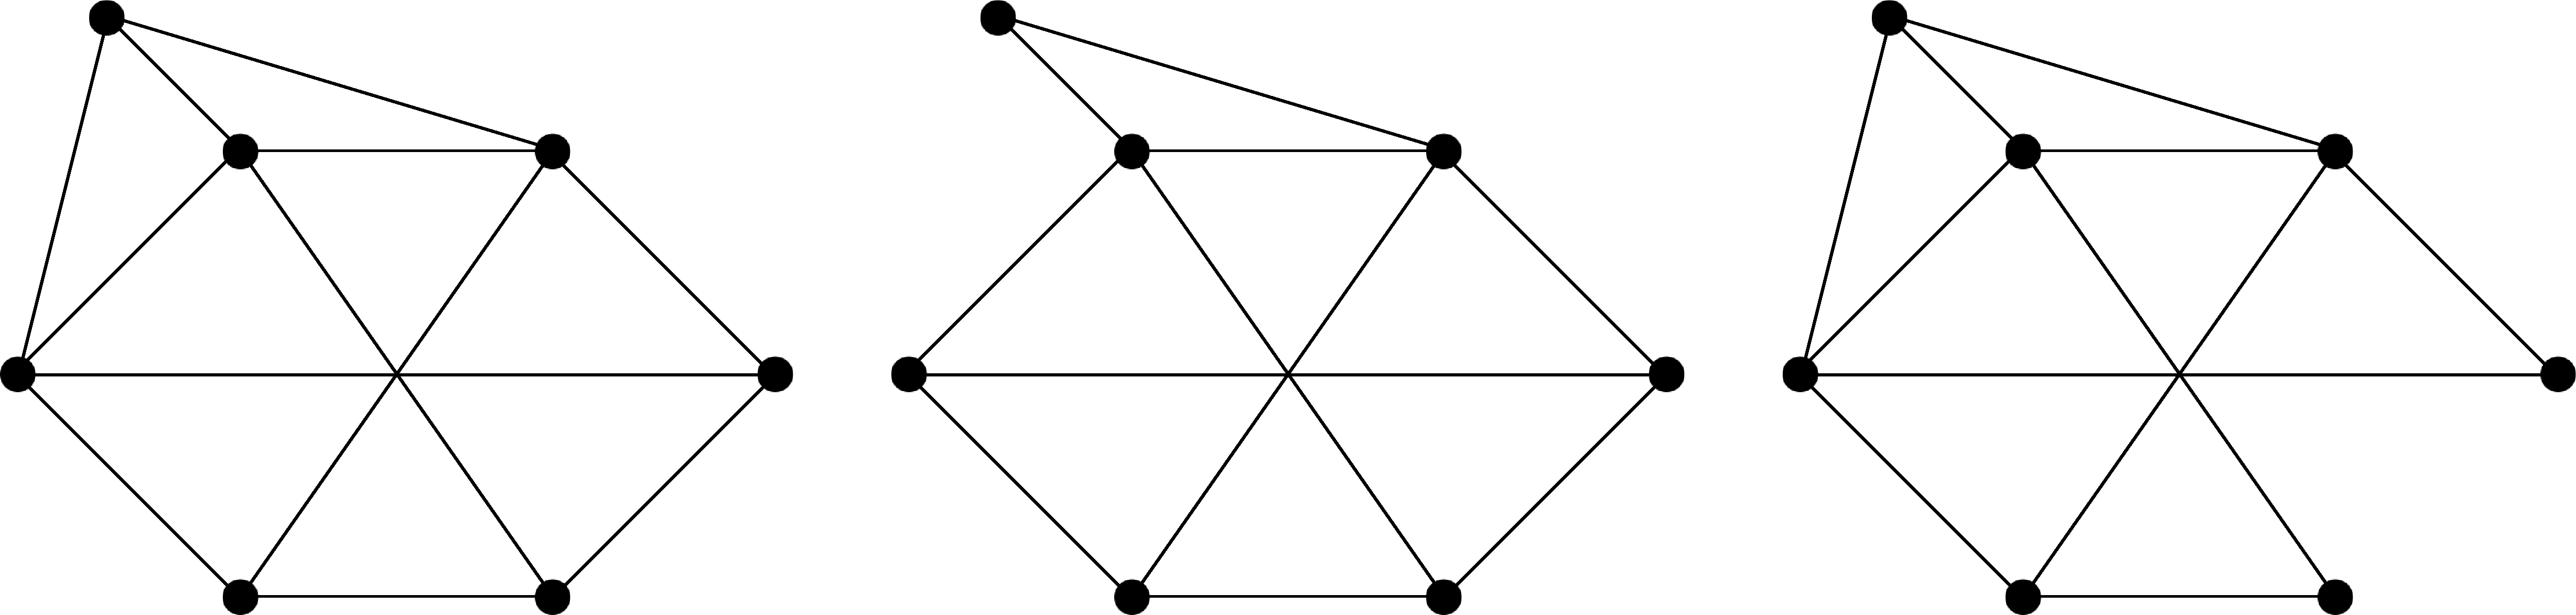
\includegraphics[width=\linewidth]{../../img/svg/overconstrained_choices}
%   \caption{The first graph is over constrained by one edge (a $K_{3,3}$ with an extra vertex attached by 3 edges). The second graph is a minimally rigid subgraph of the first. Any DR-plan of this graph will have fan-in of at least 9, occurring at the node that decomposes the $K_{3,3}$. The third graph is a different subgraph of the first. A canonical and cluster minimal DR-plan of size 2 can be made for this graph (it is a Henneberg-I construction). Thus, we can see the first graph has both non-optimal (second graph) and optimal (third graph) canonical, cluster minimal DR-plans.}
%   \label{fig:overconstrained_choices}
% \end{figure*}%



\ClearMyMinHeight
\SetMyMinHeight{.6}{../../img/svg/new_overconstrained_not_optimal}
\SetMyMinHeight{.4}{../../img/svg/new_overconstrained_optimal}

\begin{figure*}\centering%
    %
    \begin{subfigure}{0.5\linewidth}\centering
        \scalebox{1}[.9]{
        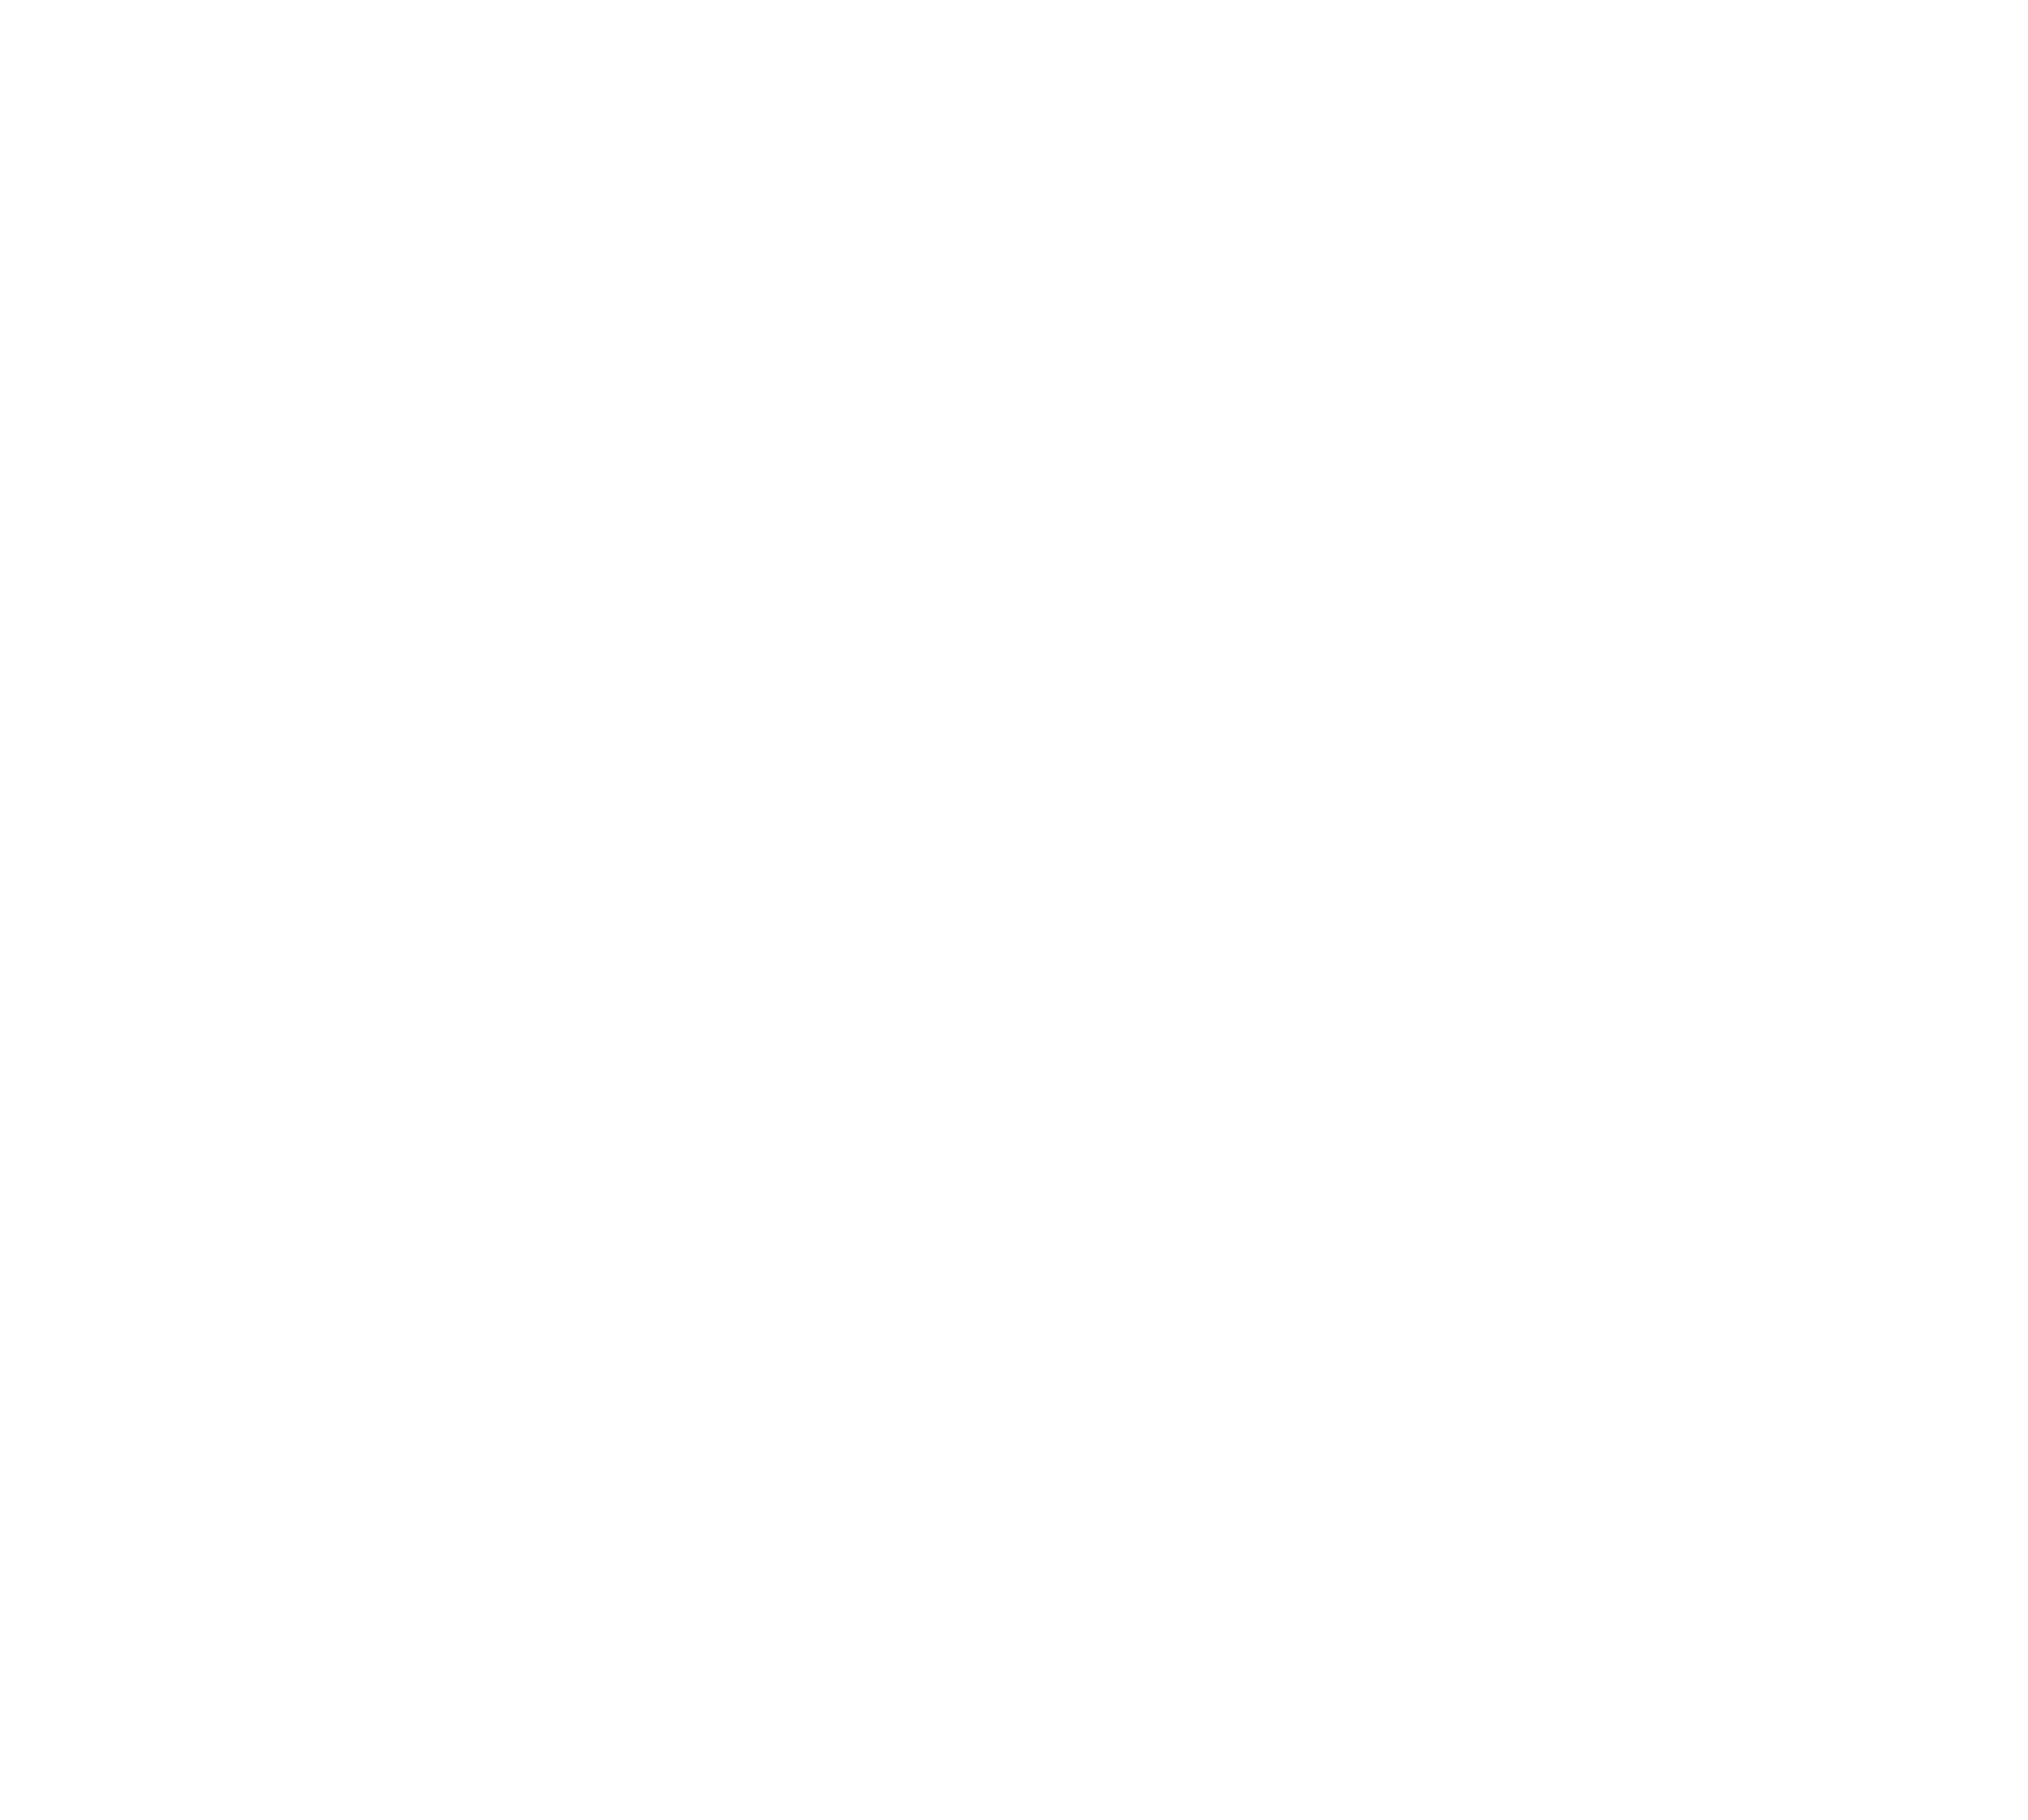
\includegraphics[height=\myMinHeight]{../../img/svg/new_overconstrained_optimal}
        }
        \caption{}\label{fig:overconstrained:optimal}
    \end{subfigure}%
    %
    \hfill
    \begin{subfigure}{0.5\linewidth}\centering
        \scalebox{1}[.9]{
        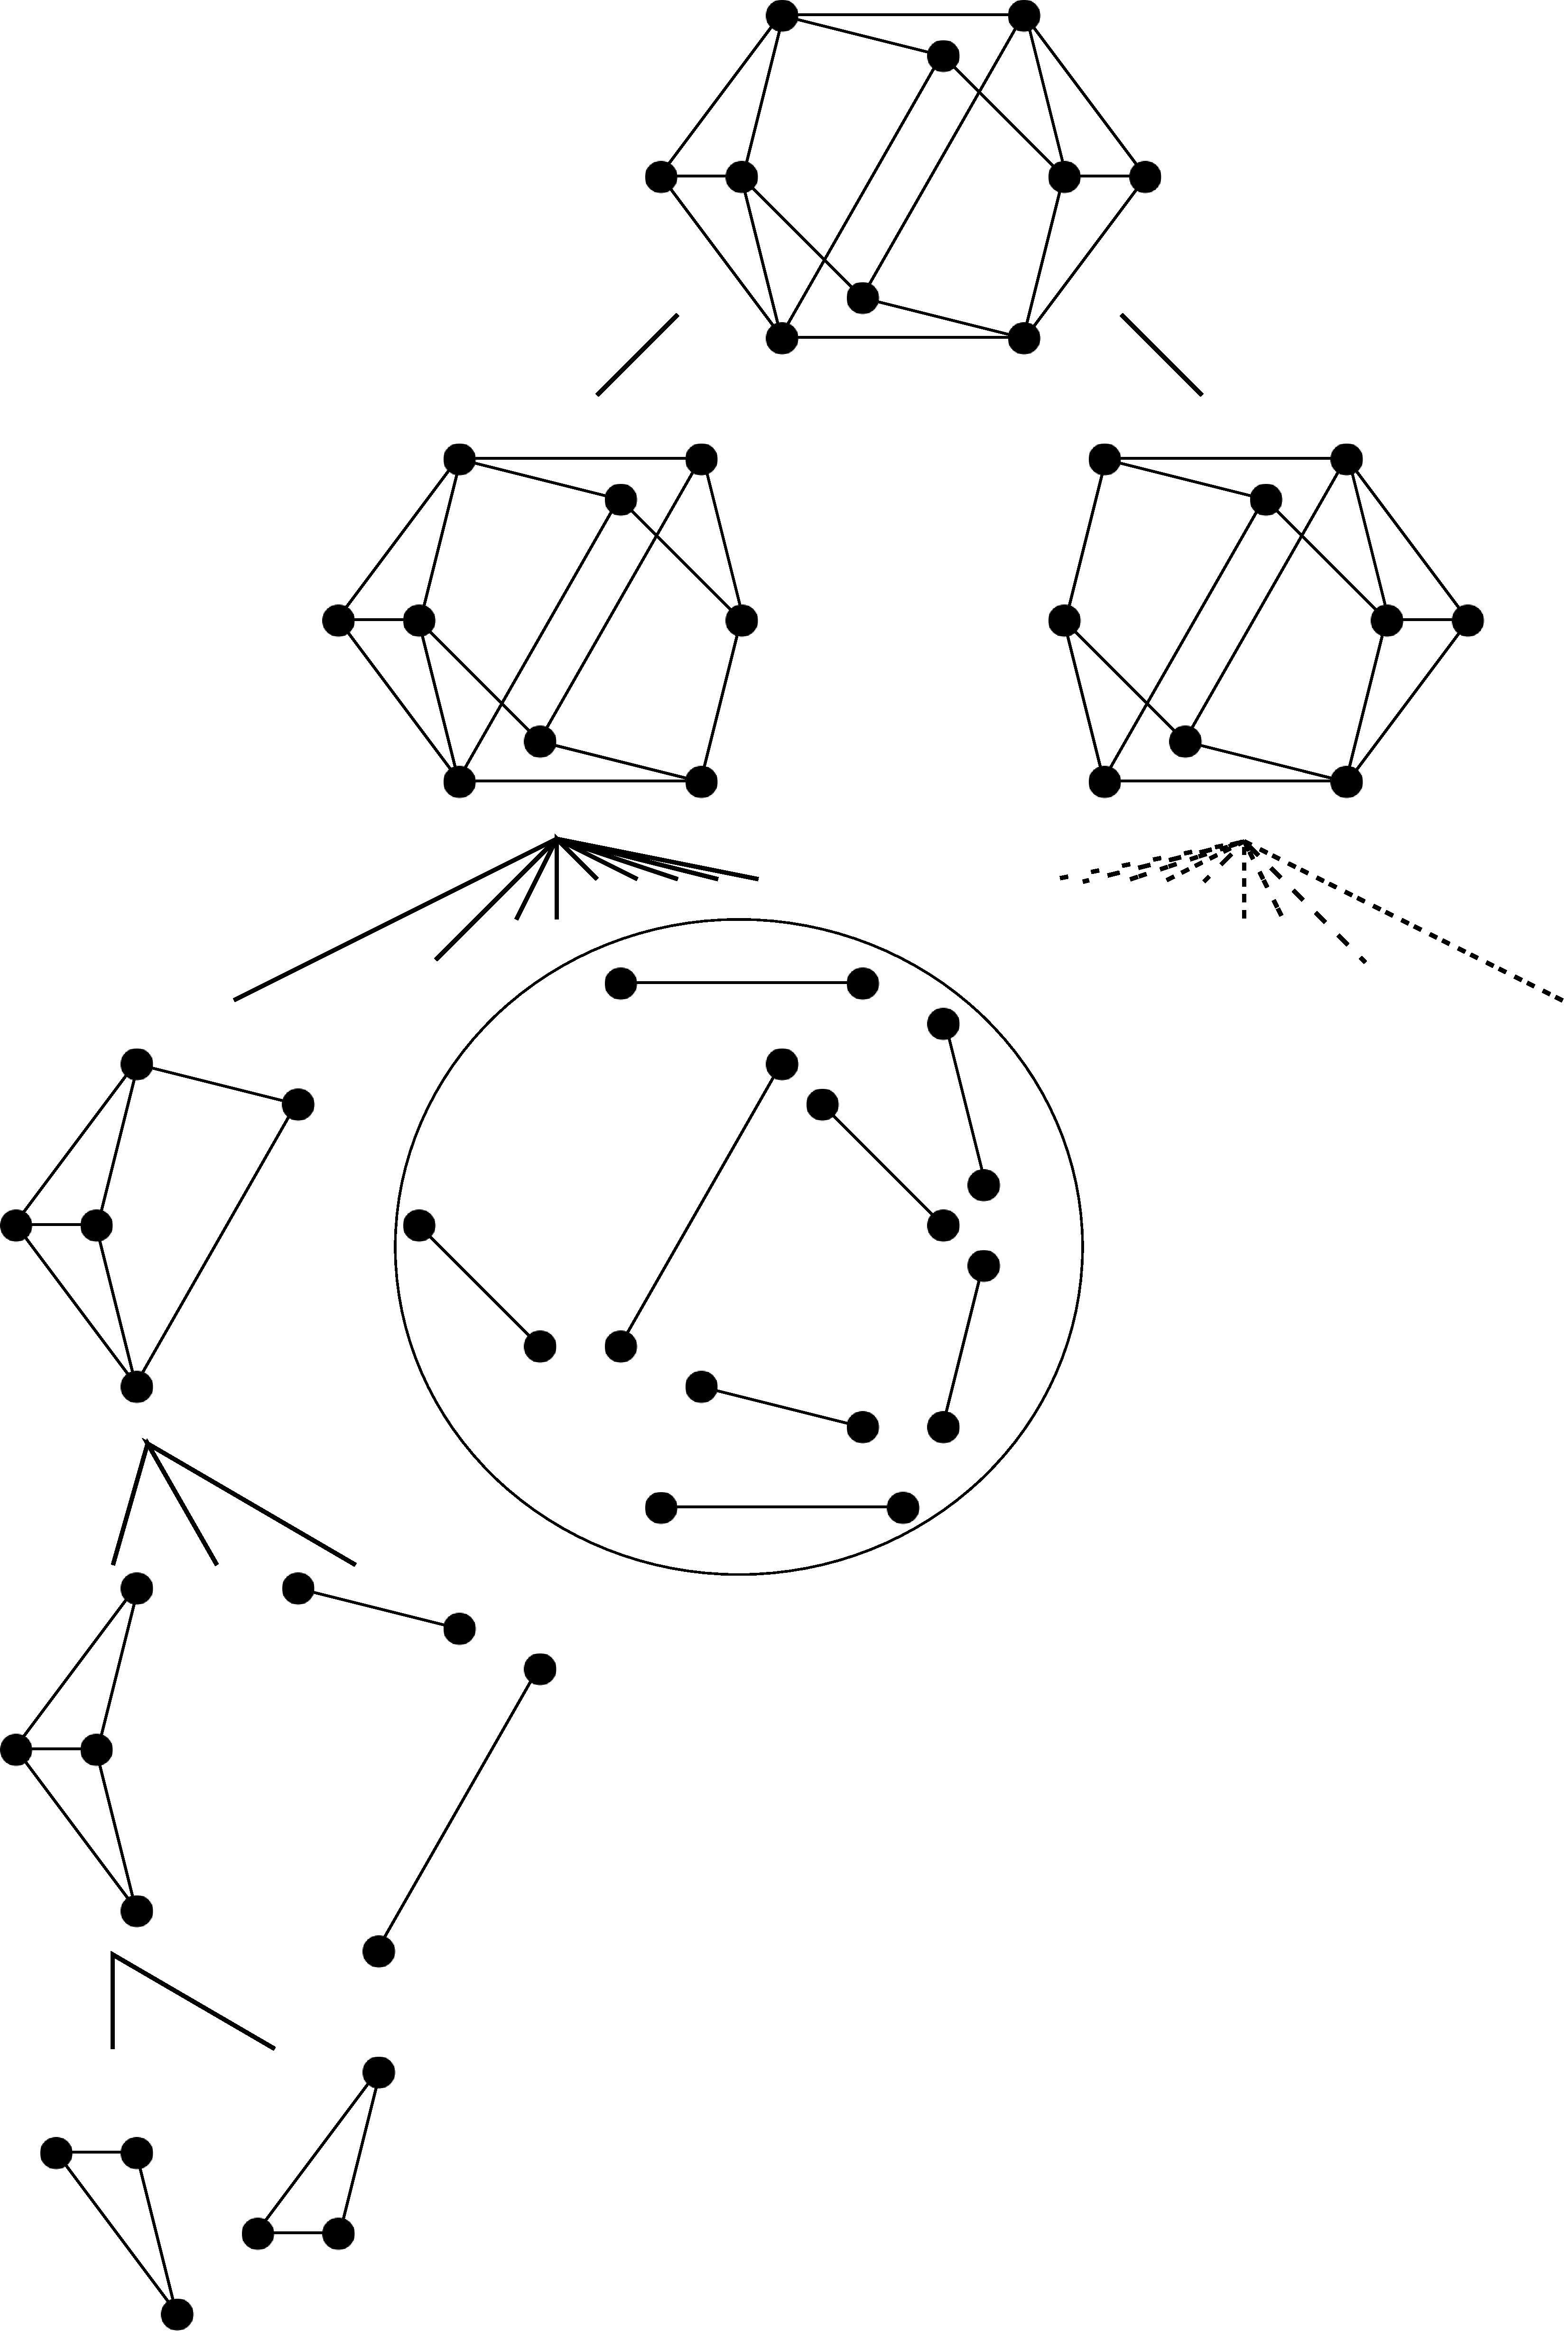
\includegraphics[height=\myMinHeight]{../../img/svg/new_overconstrained_not_optimal}
        }
        \caption{}\label{fig:overconstrained:not_optimal}
    \end{subfigure}%
    %
    \caption{
    % (\ref{fig:overconstrained:optimal}) An optimal DR-plan of a singly overconstrained rigid graph with a fan-in of 5. Decomposition of triangles is omitted. (\ref{fig:overconstrained:not_optimal}) A canonical and cluster-minimal DR-plan of the same graph. The DR-plan has a fan-in of 9 and is non-optimal, shown by the preceding counter-example. Since the nontrivial intersection of the two children of the root is underconstrained, their decompositions are separate, causing the large fan-in.
    Both figures are canonical and cluster-minimal DR-plans of the same singly overconstrained rigid graph. Decomposition of triangles are omitted and dashed lines indicate a decomposition similar to the other nodes on the same level. (\ref{fig:overconstrained:optimal}) is an optimal DR-plan, with a fan-in of 5. (\ref{fig:overconstrained:not_optimal}) has a fan-in of 9 and is non-optimal, shown by the preceding counter-example.
    }
    \label{fig:overconstrained}
\end{figure*}%


For overconstrained (not independent) graphs, a canonical DR-plan is still well-defined.
However, it may be far from optimal. The proofs of Theorem \ref{theorem:main}, Observation \ref{lemma:union_intersection}, and Lemma \ref{lemma:combined_lemma} all fail for overconstrained graphs.
It is important to note that, regardless whether the graph is overconstrained, if every node in a canonical DR-plan $R$ has clusters whose pairwise intersection is trivial, then the DR-plan is the unique one satisfying Property (2), and since we know that there is an optimal DR-plan that satisfies Property (2), $R$ is in fact optimal. The problem arises when some node in a DR-plan has clusters whose pairwise intersection is non-trivial.
In this case, an arbitrary choice of a pair of clusters as children of an overconstrained node in a canonical DR-plan may not result in an optimal DR-plan. This is in contrast to independent graphs, which, as shown in Theorem~\ref{theorem:main}, exhibit the strong Church-Rosser property that any choice yields an optimal DR-plan.
% \todo{rephrase? Theorem 4 shows this. If it's independent it \vemph{will} be optimal (the church rosser property), no longer holds if it's overconstrained.}
A good source of examples of overconstrained graphs with canonical DR-plans that are not optimal are graphs whose cluster-minimal DR-plans that are not optimal. The example shown in Figure \ref{fig:overconstrained} is a canonical, cluster-minimal DR-plan that is not optimal; an optimal DR-plan is also shown in the figure.
The root cause of the NP-hardness is encapsulated in this figure: because the different choices of vertex-maximal subgraphs for overconstrained input do not incur the same fan-in, finding the optimal DR-plan becomes a search problem with a combinatorial explosion of options.


As mentioned earlier, the Modified \frontier\ algorithm
version given in \cite{lomonosov2004graph} runs in polynomial time and finds a cluster-minimal DR-plan for any graph.
Similarly, the algorithm given above finds a canonical DR-plan also for any input graph.  However neither of these DR-plans may be optimal for overconstrained graphs as shown in Figure \ref{fig:overconstrained}.

While the canonical DR-plan is optimal only if the input graph is independent, when there are only $k$ overconstraints for some fixed $k$, we can still find the optimal DR-plan using a straightforward modification of the above algorithm. However, the time complexity is exponential in $k$.

This exponential growth of time complexity for overconstrained graphs is in fact captured in the proof of NP-hardness of optimal DR-planning in \cite{sitharam2005combinatorial, lomonosov2004graph}.
